\documentclass[unicode,11pt,a4paper,oneside,numbers=endperiod,openany]{scrartcl}

% Required package
\usepackage{amssymb}
\usepackage{graphicx}
\usepackage{amsmath}
\usepackage{matlab-prettifier}
\usepackage{float}
\usepackage[export]{adjustbox}
\usepackage{multirow}
\usepackage{booktabs}

\renewcommand{\thesubsection}{\arabic{subsection}}

% vector shortcut
\newcommand{\myvec}[1]{\begin{bmatrix} #1 \end{bmatrix}}
\newcommand{\myex}[1]{\begin{equation*}\begin{aligned} #1 \end{aligned}\end{equation*}}
\newcommand{\myexthreeA}{\myvec{2 & 0 \\ 0 & 2\mu}}

\usepackage{ifthen}
\usepackage[utf8]{inputenc}
\usepackage{graphics}
\usepackage{graphicx}
\usepackage{hyperref}
\usepackage{amsmath}

\pagestyle{plain}
\voffset -5mm
\oddsidemargin  0mm
\evensidemargin -11mm
\marginparwidth 2cm
\marginparsep 0pt
\topmargin 0mm
\headheight 0pt
\headsep 0pt
\topskip 0pt        
\textheight 255mm
\textwidth 165mm

\newcommand{\duedate} {}
\newcommand{\setduedate}[1]{%
\renewcommand\duedate {\textbf{Due date:}~ #1}}
\newcommand\isassignment {false}
\newcommand{\setassignment}{\renewcommand\isassignment {true}}
\newcommand{\ifassignment}[1]{\ifthenelse{\boolean{\isassignment}}{#1}{}}
\newcommand{\ifnotassignment}[1]{\ifthenelse{\boolean{\isassignment}}{}{#1}}

\newcommand{\assignmentpolicy}{
\begin{table}[h]
\begin{center}
\scalebox{0.8} {%
\begin{tabular}{|p{0.02cm}p{16cm}|}
\hline
&\\
\multicolumn{2}{|c|}{\Large\textbf{Numerical Computing 2023 ---  Submission Instructions}}\\
\multicolumn{2}{|c|}{\large\textbf{(Please, notice that following instructions are mandatory: }}\\
\multicolumn{2}{|c|}{\large\textbf{submissions that don't comply with, won't be considered)}}\\
&\\
\textbullet & Assignments must be submitted to \href{https://www.icorsi.ch/course/view.php?id=14666}{iCorsi} (i.e. in electronic format).\\
\textbullet & Provide both executable package and sources (e.g. C/C++ files, MATLAB). 
If you are using libraries, please add them in the file. Sources must be organized in directories called:\\
\multicolumn{2}{|c|}{\textit{Project\_number\_lastname\_firstname}}\\
& and  the  file must be called:\\
\multicolumn{2}{|c|}{\textit{project\_number\_lastname\_firstname.zip}}\\
\multicolumn{2}{|c|}{\textit{project\_number\_lastname\_firstname.pdf}}\\
\textbullet &  The TAs will grade your project by reviewing your project write-up, and looking at the implementation you attempted, and benchmarking your code's performance.\\

\textbullet & You are allowed to discuss all questions with anyone you like; however: (i) your submission must list anyone you discussed problems with and (ii) you must write up your submission independently.\\
\hline
\end{tabular}
}
\end{center}
\end{table}
}
\newcommand{\punkte}[1]{\hspace{1ex}\emph{\mdseries\hfill(#1~\ifcase#1{Points}\or{Points}\else{Points}\fi)}}


\newcommand\serieheader[6]{
\thispagestyle{empty}%
\begin{flushleft}

\includegraphics[width=0.45\textwidth]{CI_logo}
\end{flushleft}
  \noindent%
  {\large\ignorespaces{\textbf{#1}}\hspace{\fill}\ignorespaces{ \textbf{#2}}}\\ \\%
  {\large\ignorespaces #3 \hspace{\fill}\ignorespaces #4}\\
  \noindent%
  \bigskip
  \hrule\par\bigskip\noindent%
  \bigskip {\ignorespaces {\Large{\textbf{#5}}}
  \hspace{\fill}\ignorespaces \large \ifthenelse{\boolean{\isassignment}}{\duedate}{#6}}
  \hrule\par\bigskip\noindent%  \linebreak
 }

\makeatletter
\def\enumerateMod{\ifnum \@enumdepth >3 \@toodeep\else
      \advance\@enumdepth \@ne
      \edef\@enumctr{enum\romannumeral\the\@enumdepth}\list
      {\csname label\@enumctr\endcsname}{\usecounter
        {\@enumctr}%%%? the following differs from "enumerate"
	\topsep0pt%
	\partopsep0pt%
	\itemsep0pt%
	\def\makelabel##1{\hss\llap{##1}}}\fi}
\let\endenumerateMod =\endlist
\makeatother




\usepackage{textcomp}





\begin{document}


\setassignment
\setduedate{Friday, 12 April 2024, 12:00 AM}

\serieheader
{Optimization Methods}
{2024}
{\textbf{Student:} Jeferson Morales Mariciano \\\\}
{\textbf{Discussed with:} Leonardo Birindelli}
{Assignment 2}{}
\newline

%\assignmentpolicy


% EXERCISE 1 %%%%%%%%%%%%%%%%%%%%%%%%%%%%%%%%%%%%%%%%%%%%%%%%%%%%%%%%%%%%%%%%%%%%%%%%%%%%%%%%%%%%%%
\section*{Exercise 1}
Considering the highly non-linear Rosenbrock's function:
\begin{equation} \label{eq:rosenbrock}
    f(x, y) := (1 - x)^2 + 100(y - x^2)^2 
\end{equation}

\subsection*{1, 2, 3}
Implement in MATLAB two functions: 
Newton's method (Newton.m), Steepest descent (Gradient) method (GD.m).
Both methods can be run with backtracking algorithm (backtracking.m) with step size $\beta = 1$. 
Use the following values for the backtracking parameters: 
$\tilde{\alpha} = 1, \rho = 0.9$. 
You can choose the parameter $c_1 \in [0.5, 10^{-4}]$.

Minimize the Rosenbrock's function \ref{eq:rosenbrock} 
by using the Steepest Descent (Gradient) method with backtracking and fixed step size $\beta = 1$. 
Use starting value $x_0 = (0, 0)$, 
maximum number of iterations $N = 50000$ and tolerance $TOL = 10^{-6}$.

Minimize the Rosenbrock's function \ref{eq:rosenbrock} 
by using Newton method with backtracking and fixed step size $\beta = 1$. 
Use same parameters as for SD.
\\\newline
Matlab scripts are provided in \textit{/code} folder.
The 2 main files to run are: \textit{GD.m, Newton.m}.

\subsection*{4, 5, 6}
Plot the obtained iterates on the energy landscape in 2D.
Analyze convergence behaviour of the methods by plotting the gradient norm and the function
value at each iteration.
Compare and comment on the the performances of the different methods.
\\\newline
\begin{figure}[H]
    \centering
    \caption{Visualization of Steepest Descent}
    \label{fig:ex1-sd-energy}
    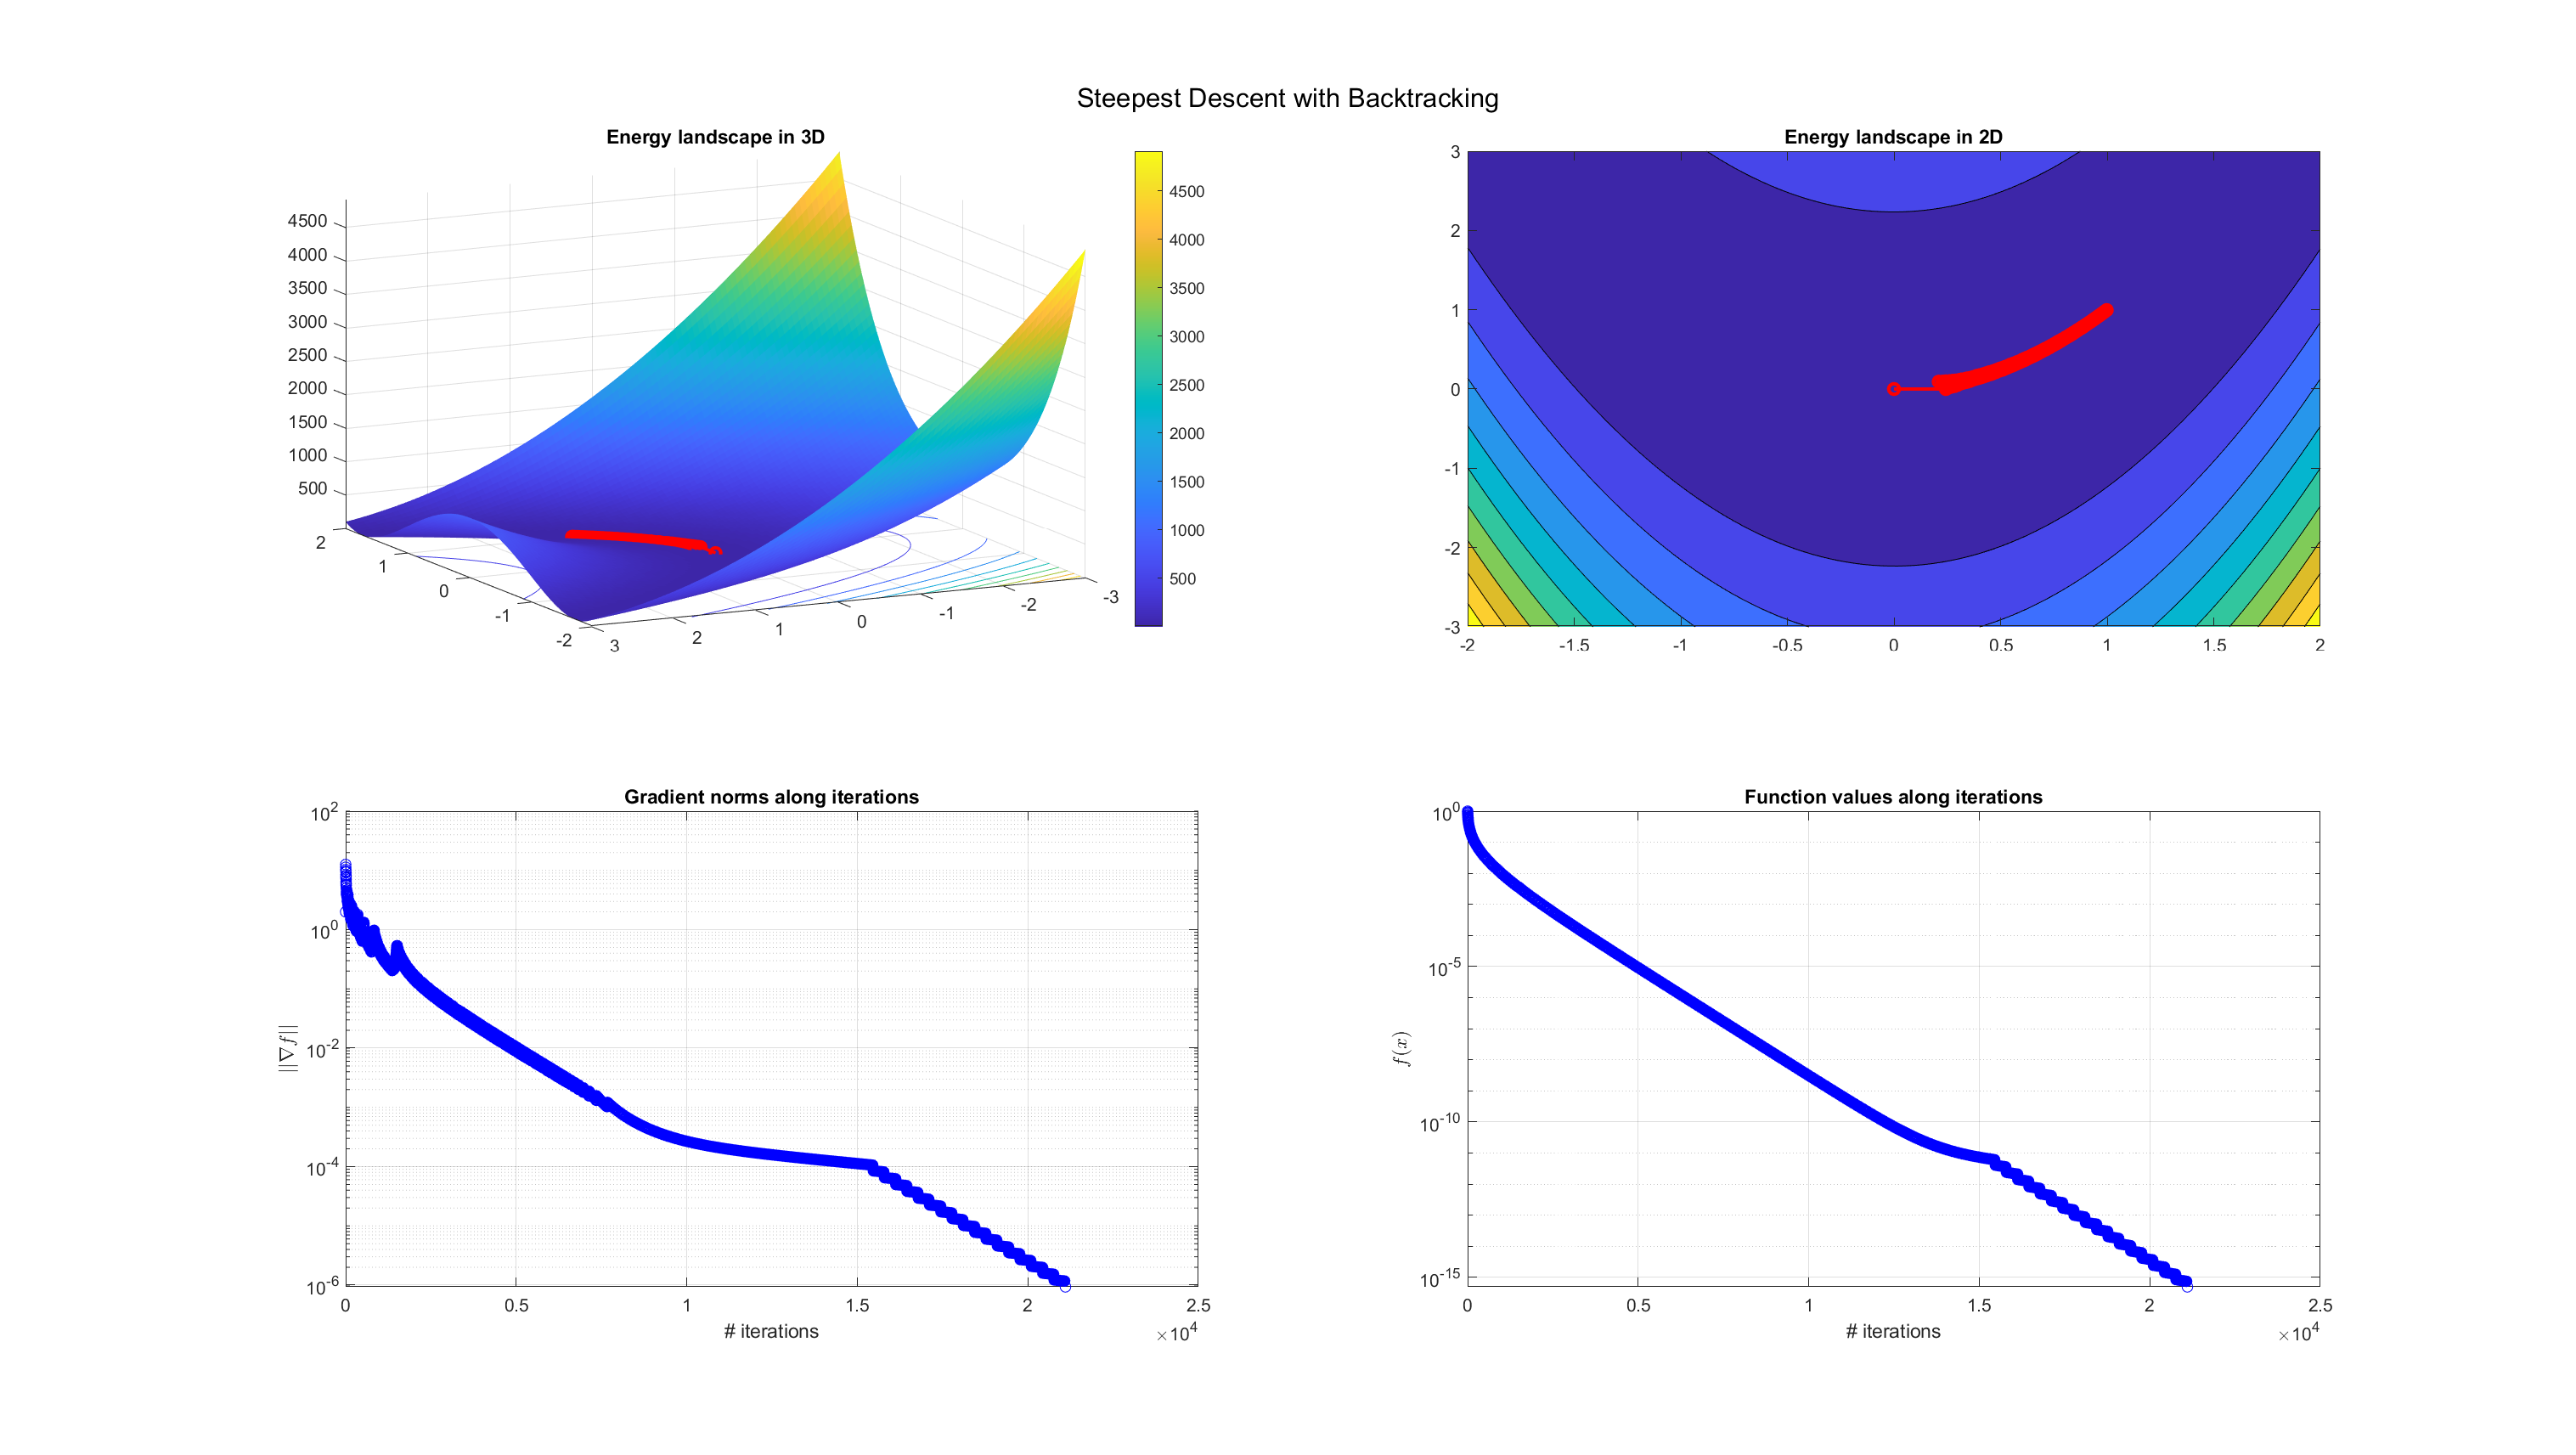
\includegraphics[width=\textwidth, trim={4cm 2.5cm 4cm 1.5cm}, clip]{./figures/ex1-sd-backtracking-energy.eps}
\end{figure}

\begin{figure}[H]
    \centering
    \caption{Comparison of convergence}
    \label{fig:ex1-convergence-comparison}
    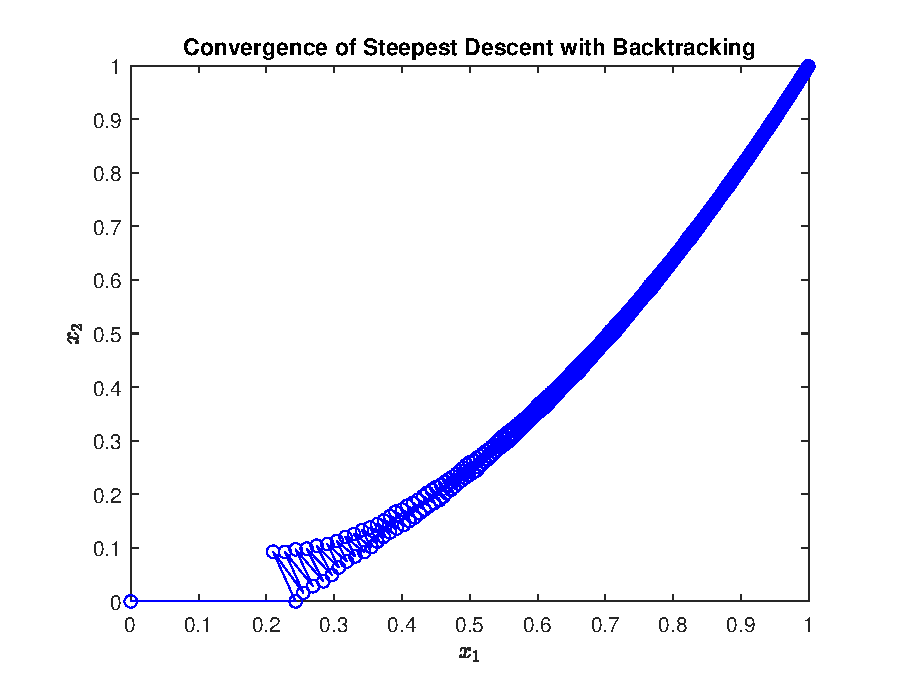
\includegraphics[width=.5\textwidth, trim={0cm 0cm 0cm 0cm}, clip]{./figures/ex1-sd-backtracking-convergence.eps}
    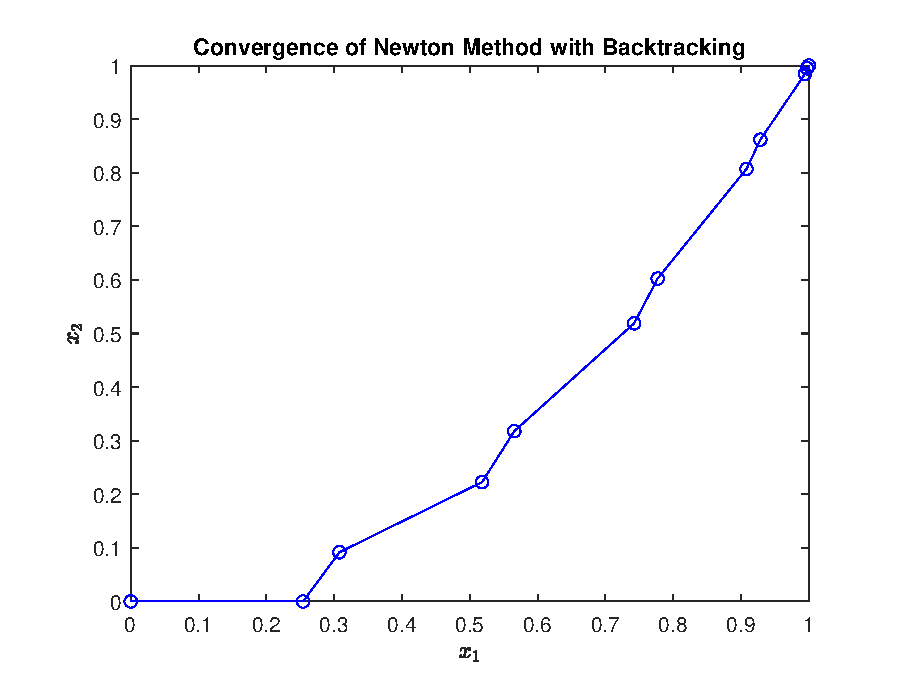
\includegraphics[width=.49\textwidth, trim={0cm 0cm 0cm 0cm}, clip]{./figures/ex1-newton-backtracking-convergence.eps}
\end{figure}

\begin{figure}[H]
    \centering
    \caption{Visualization of Newton Method}
    \label{fig:ex1-newton-energy}
    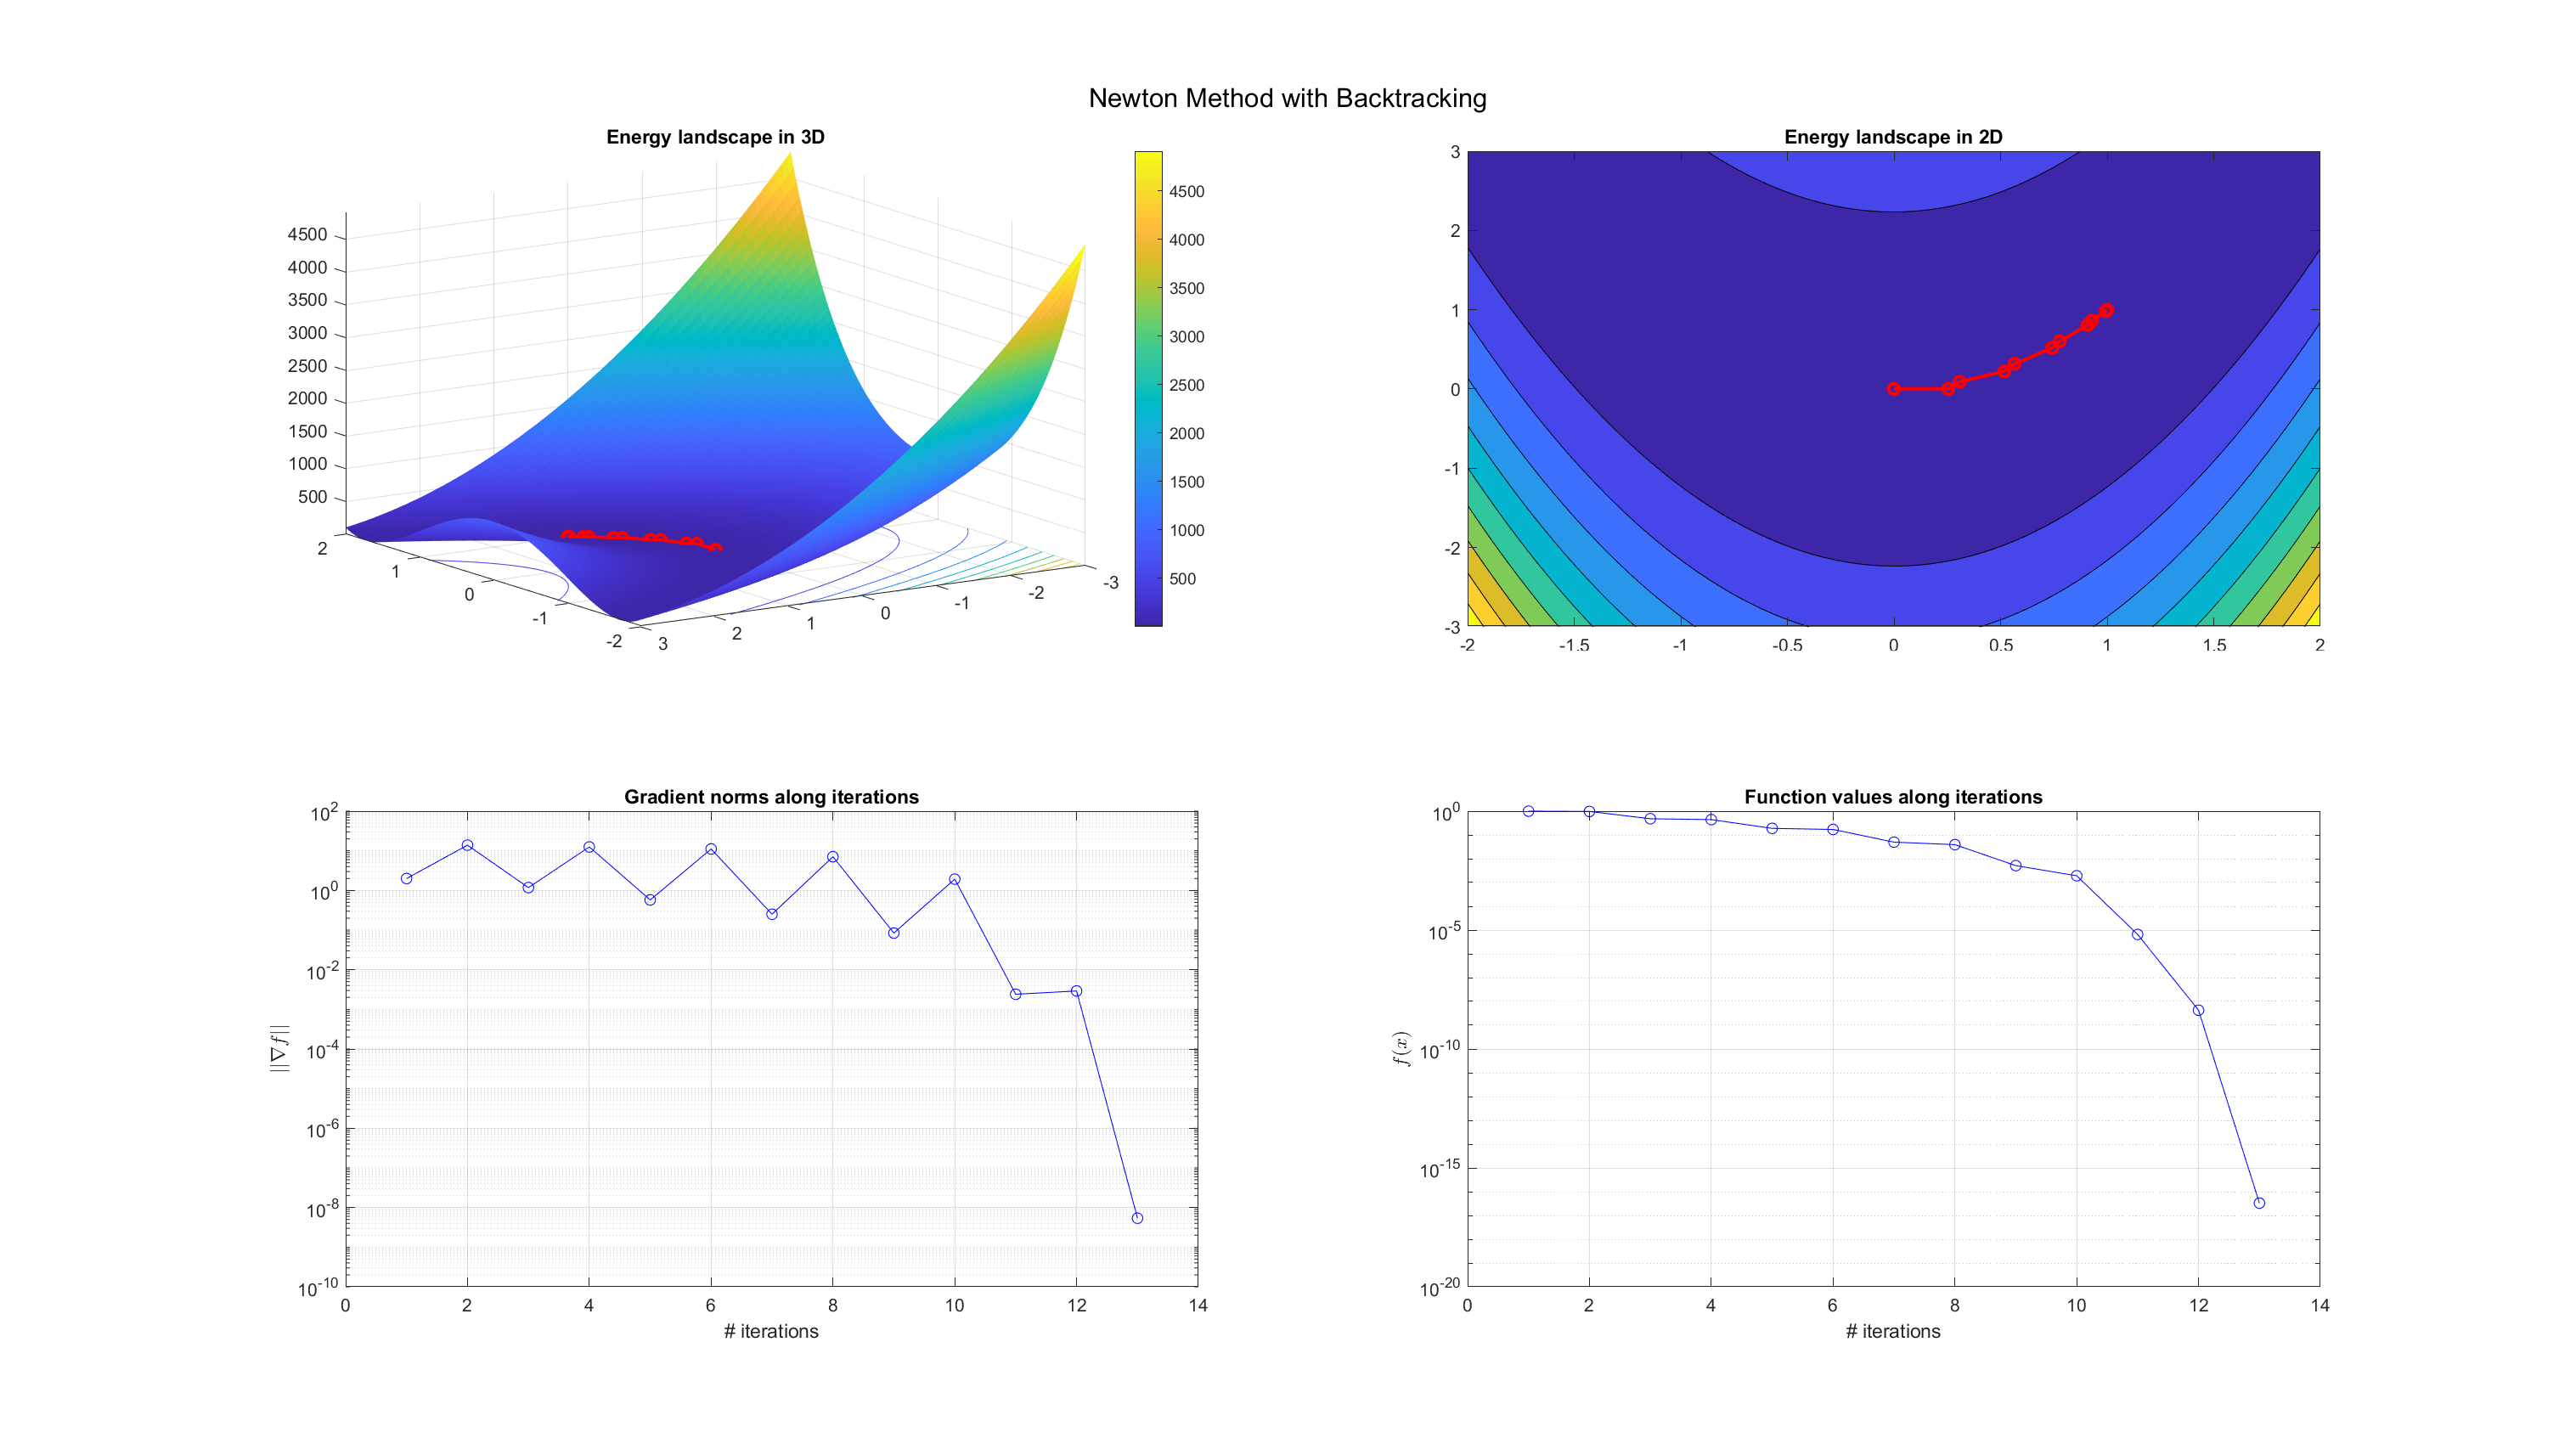
\includegraphics[width=\textwidth, trim={4cm 2.5cm 4cm 1.5cm}, clip]{./figures/ex1-newton-backtracking-energy.eps}
\end{figure}

Chosen $c_1 = 1e-4$. 


% Vector-valued function $f : \mathbb{R}^2 \rightarrow \mathbb{R}$

% \begin{equation}
%     f(x_1, x_2) = 200 (x_2 - x_1^2)^2 + (1 - x_1)^2
% \end{equation}

% \subsection{}
% Compute gradient $\nabla f : \mathbb{R}^2 \rightarrow \mathbb{R}^2$
% and Hessian $H_f : \mathbb{R}^2 \rightarrow \mathbb{R}^{2 \times 2}$. \newline

% \begin{equation*}
% \begin{aligned}
%     \begin{bmatrix} x_1 \\ x_2 \end{bmatrix}
%      & \mapsto 200 (x_2 - x_1^2) (x_2 - x_1^2) + (1 - x_1) (1 - x_1) \\
%      & = 200 (x_2^2 - 2x_2 x_1^2 + x_1^4) + (1 - 2x_1 + x_1^2)       \\
%      & = 200 x_2^2 - 400 x_2 x_1^2 + 200 x_1^4 + 1 - 2x_1 + x_1^2    \\
%     \nabla f
%      & = \begin{bmatrix}
%              \frac{\partial f}{\partial x_1} \\
%              \frac{\partial f}{\partial x_2}
%          \end{bmatrix}
%         = \begin{bmatrix}
%           -800 x_2 x_1 + 800 x_1^3 + 2x_1 - 2 \\
%           400 x_2 - 400 x_1^2
%         \end{bmatrix} \\
%     H_f
%      & =\begin{bmatrix}
%             \frac{\partial^2 f}{\partial x_1^2}            
%             & \frac{\partial^2 f}{\partial x_1 \partial x_2} \\
%             \frac{\partial^2 f}{\partial x_2 \partial x_1} 
%             & \frac{\partial^2 f}{\partial x_2^2}            \\
%         \end{bmatrix}
%         = \begin{bmatrix}
%           -800 x_2 + 2400 x_1^2 + 2 & - 800 x_1 \\
%           -800 x_1                  & 400
%         \end{bmatrix}
% \end{aligned}
% \end{equation*}

% \subsection{}
% Write Taylor's expansion of $f$ up to 2nd order around point
% $(x_1, x_2) = (0, 0)$. \newline

% Given $x_0 = (0, 0)$, $f(x_0) = 1$, 
% $\nabla f(x_0) = \begin{bmatrix} -2 \\ 0 \end{bmatrix}$, 
% $H_f(x_0) = \begin{bmatrix} 2 & 0 \\ 0 & 400 \end{bmatrix}$, 
% incognites $h = \begin{bmatrix} x_1 \\ x_2 \end{bmatrix}$

% \begin{equation*}
% \begin{aligned}
%     f(x_0 + h)
%      & = f(x_0) + h^T \nabla f(x_0) + \frac{1}{2} h^T H_f(x_0) h + o(|| h ||^2)                                                                                                                                                                                                                                                                                      \\
%      & = 1 + \myvec{x_1 & x_2} \myvec{-2 \\ 0 } + \frac{1}{2} \myvec{x_1 & x_2} \myvec{2 & 0 \\ 0 & 400} \myvec{x_1 \\ x_2} + o(|| h ||^2) \\
%      & = 1 - 2x_1 + \frac{1}{2} \myvec{2x_1 & 400x_2} \myvec{x_1 \\ x_2} + o(|| h ||^2) \\ 
%      & = 1 - 2x_1 + x_1^2 + 200x_2^2 + o(|| h ||^2) \approx f(x_1, x_2)
% \end{aligned}
% \end{equation*}

% EXERCISE 2 %%%%%%%%%%%%%%%%%%%%%%%%%%%%%%%%%%%%%%%%%%%%%%%%%%%%%%%%%%%%%%%%%%%%%%%%%%%%%%%%%%%%%%
\section*{Exercise 2}


\subsection*{1, 2}
Implement the BFGS method (BFGS.m) with backtraking for the step size $\beta$. 
Test your implementation by minimizing the Rosenbrock's function. 
Use starting values $x_0 = (0, 0)$, 
$H_0 = I$, 
maximum number of iterations $N = 500$ and tolerance $TOL = 10^{-6}$.
\\\newline
Matlab scripts are provided in \textit{/code} folder.
The main file to run is \textit{BFGS.m}.

\subsection*{3, 4}
Plot the obtained iterates on the energy landscape in 2D.
Analyze convergence behaviour of the methods by plotting the gradient norm and the function
value at each iteration.

\begin{figure}[H]
    \centering
    \caption{Visualization of BFGS}
    \label{fig:ex2-bfgs-energy}
    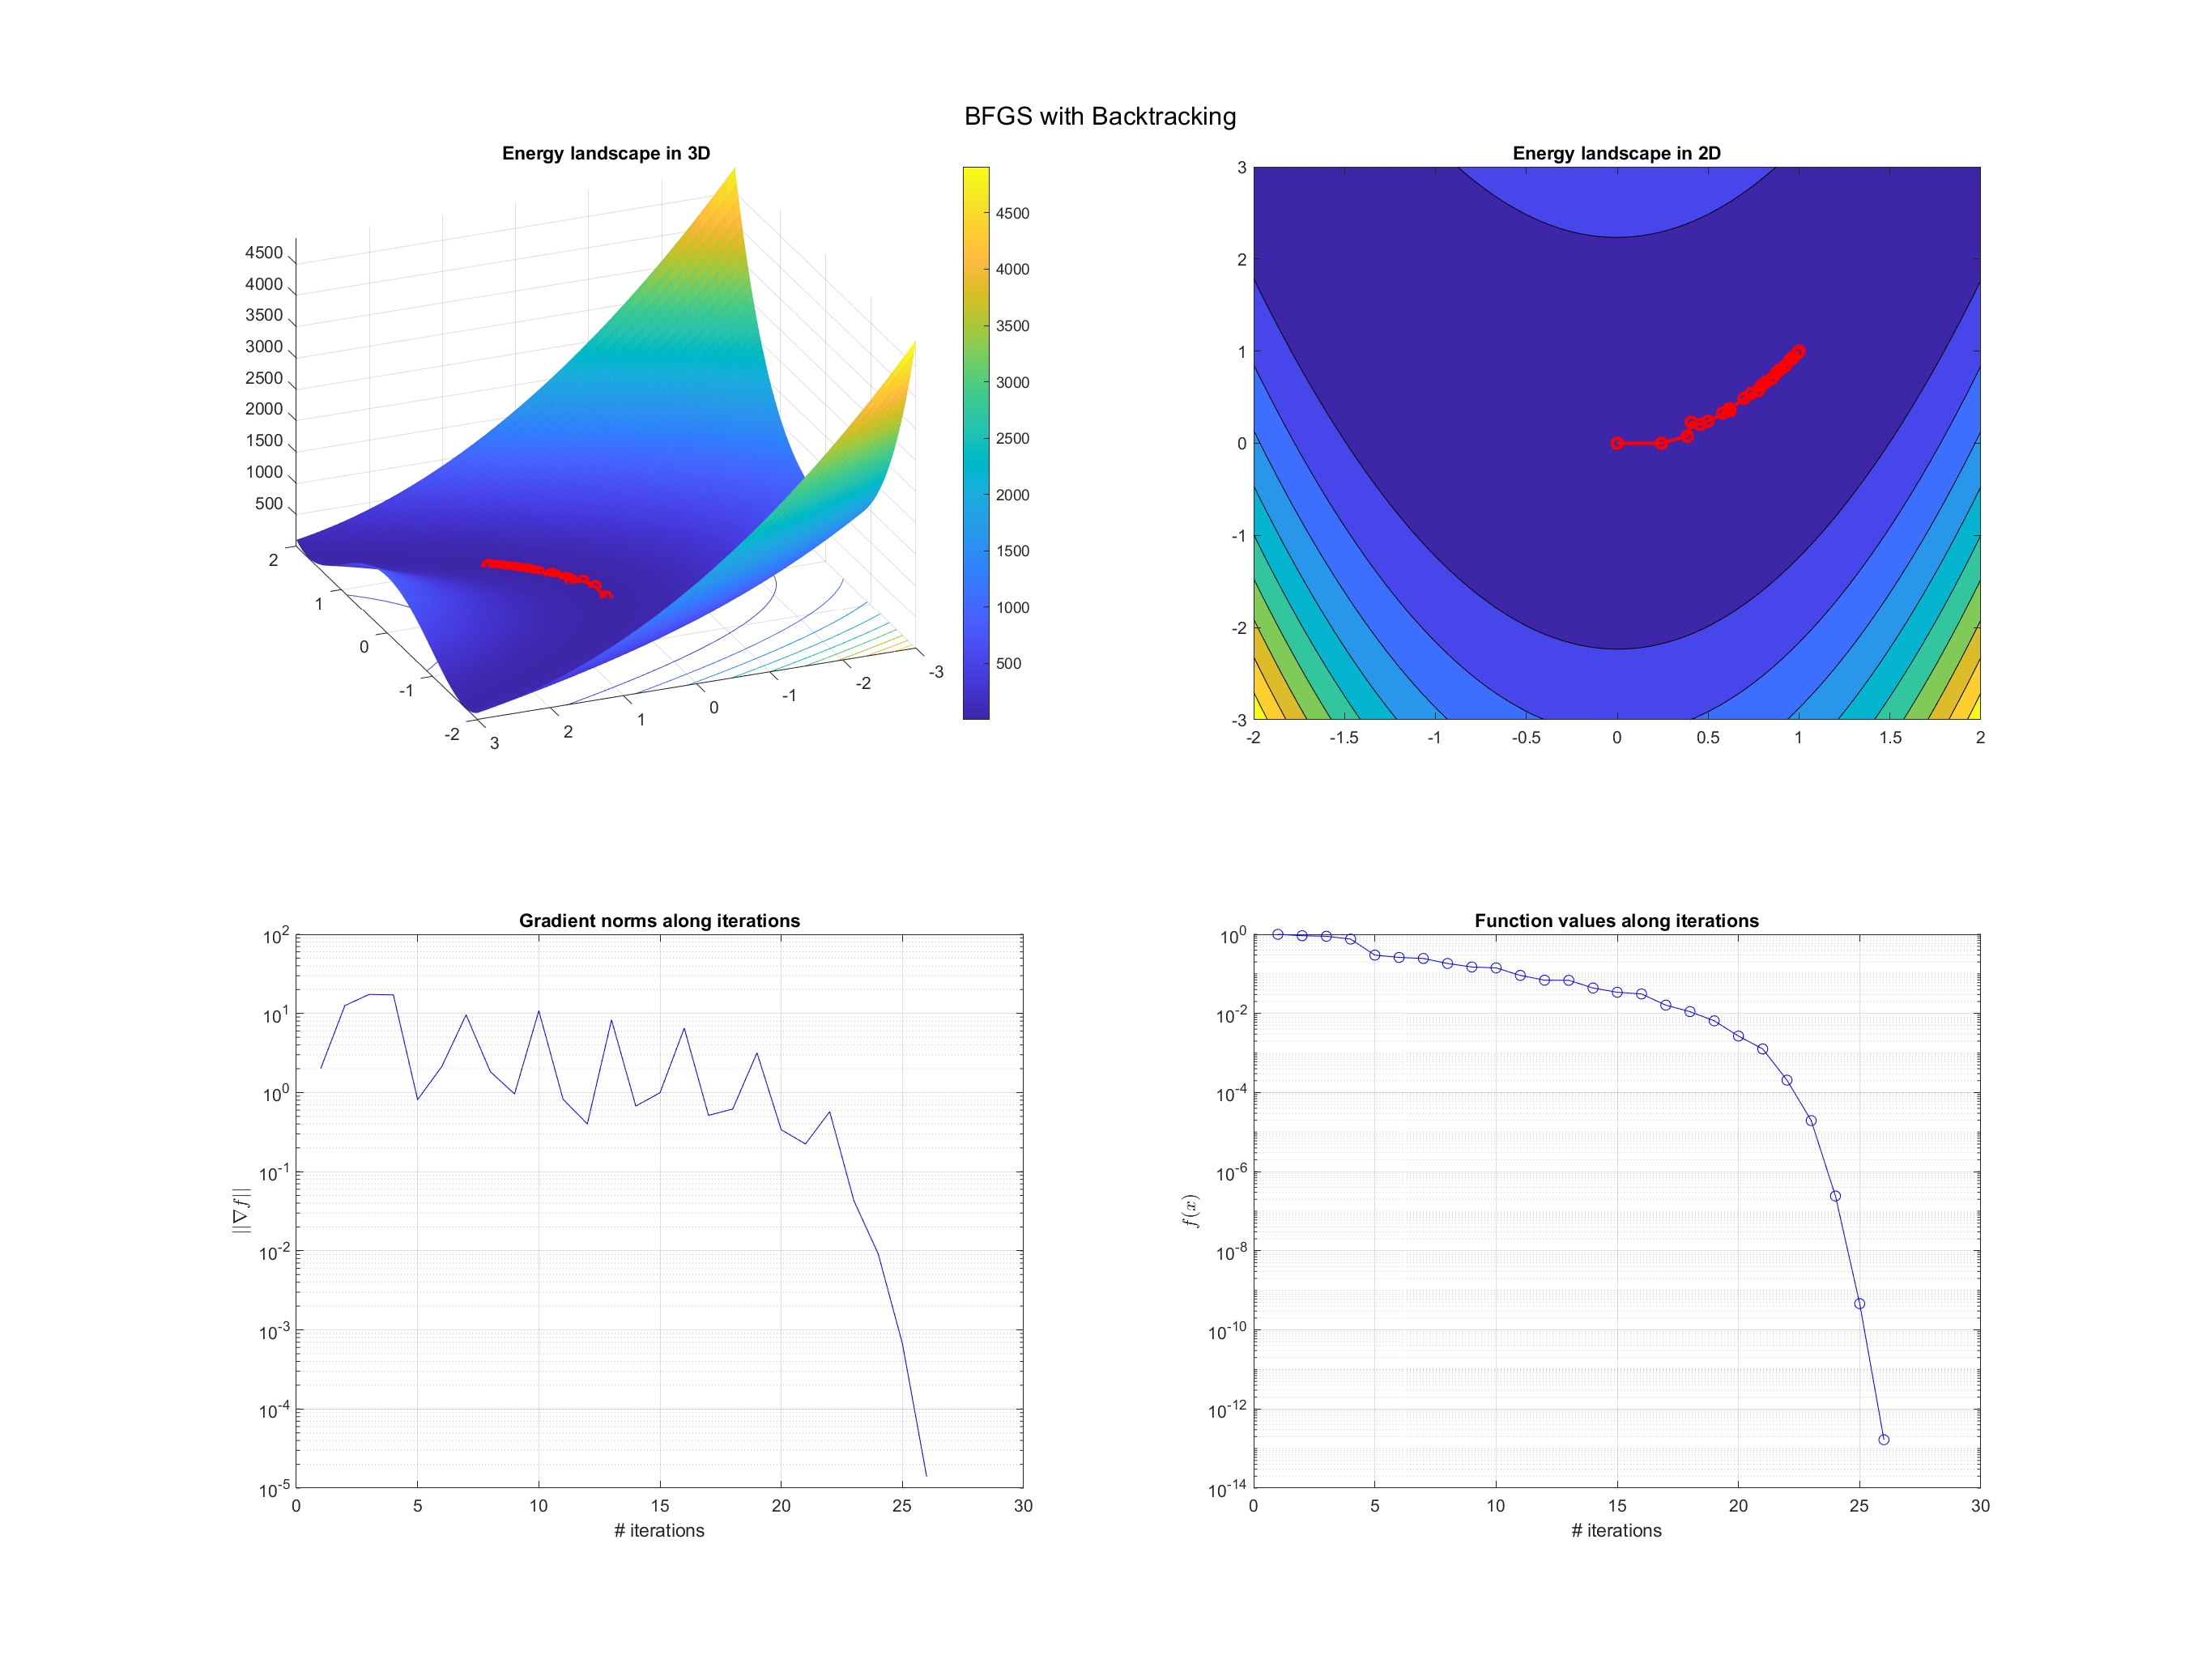
\includegraphics[width=\textwidth, trim={4cm 2.5cm 4cm 1.5cm}, clip]{./figures/ex2-bfgs-energy.eps}
\end{figure}

\begin{figure}[H]
    \centering
    \caption{Convergence of BFGS}
    \label{fig:ex2-bfgs-convergence}
    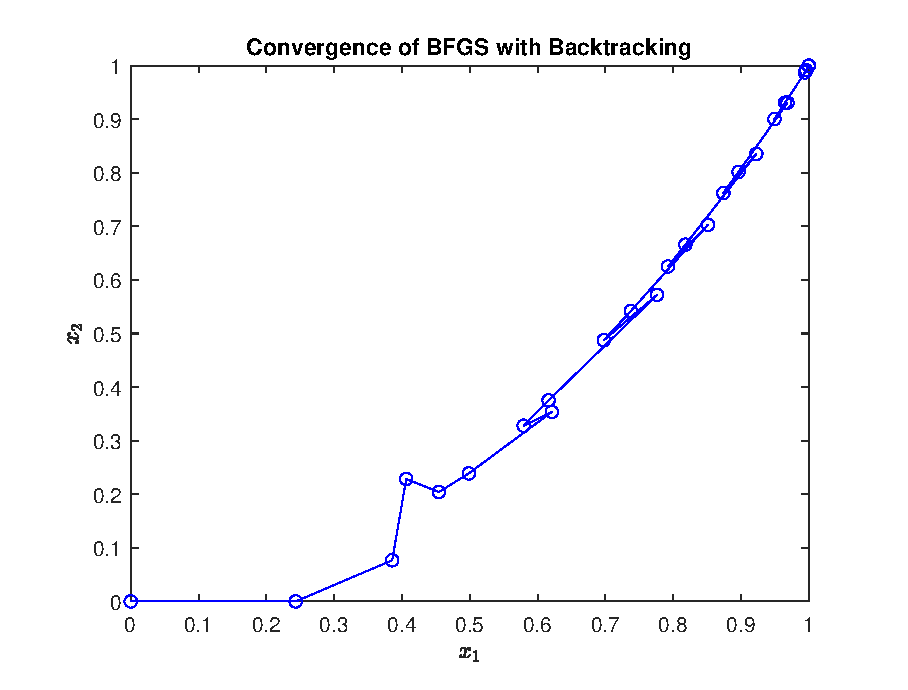
\includegraphics[width=.5\textwidth, trim={0cm 0cm 0cm 0cm}, clip]{./figures/ex2-bfgs-convergence.eps}
\end{figure}

\subsection*{5}
Produce a table in which you compare the number of iterations required by BFGS, by Newton's
method (with backtracking) and by Steepest descent method (with backtracking). You can use the
results from the previous exercise. Comment the results by comparing the different methods.

\begin{table*} \centering
\caption{Comparison of Iterations for Rosenbrock's Function}
\begin{tabular}{@{}ccc@{}}
    \toprule
    Steepest Descent & Newton & BFGS \\
    \midrule
    21102 & 12  & 26 \\
    \bottomrule
\end{tabular}
\end{table*}


% Quadratic minimization problem with $A \in \mathbb{R}^{n \times n}$ is SPD 
% $\land \, x,b \in \mathbb{R}^n$.

% \begin{equation}
%     \min_{x \in \mathbb{R}^n} J(x) = \frac{1}{2} x^T A x - b^T x
% \end{equation}

% \subsection{}
% Compute gradient and Hessian of $J$. \newline

% \myex{
%     \nabla J(x) = A \myvec{x_1 \\ \vdots \\ x_n} - b = Ax - b
% }

% \myex{
%     H_J(x) = A
% }

% \subsection{}
% Write down the 1st Order Necessary Conditions. \newline

% If $x^*$ is local minimizer 
% $\land$ $f$ continuously differentiable in open neighborhood $\mathcal{N}(x^*)$ 
% $\therefore$ $\nabla f(x^*) = 0$. 
% $x^*$ stationary point $\because$ $\nabla f(x^*) = 0$, 
% from Th 2.2 any local minimizer is a stationary point.

% \myex{
%     \nabla f(x^*) = 0 
%     \Rightarrow \nabla J(x^*) = A x^* - b
%     \Rightarrow A x^* - b = 0
%     \Rightarrow A x^* = b
% }

% \subsection{}
% Write down the 2nd Order Necessary and Sufficient Conditions. \newline

% \textbf{2nd Order Necessary Conditions}:
% If $x^*$ local minimizer of $f$ 
% $\land$ $\exists \nabla^2 f$ continuous in open neighborhood $\mathcal{N}(x^*)$ 
% $\therefore$ $\nabla f(x^*) = 0$ 
% $\land$ $\nabla^2 f(x^*)$ is positive semidefinite.

% \myex{
%     \nabla f(x^*) = 0
%     \Rightarrow \nabla J(x^*) = A x^* - b
%     \Rightarrow A x^* = b
% }
% \myex{
%     \nabla^2 f(x^*)
%     \Rightarrow \nabla^2 J(x^*) = H_J = A \text{ positive semidefinite } 
%     \therefore \text{ eigenvals } \lambda \geq 0 \,\, \forall \lambda \in \Lambda \,
%     \land \, x^T A x \geq 0
% }
% \newline

% \textbf{2nd Order Sufficient Conditions}:
% Suppose $\nabla^2 f$ continuous in open neighborhood $\mathcal{N}(x^*)$ 
% $\land$ $\nabla f(x^*) = 0$ 
% $\land$ $\nabla^2 f(x^*)$ positive definite
% $\therefore$ $x^*$ strict local minimizer of $f$.

% \myex{
%     \nabla f(x^*) = 0
%     \Rightarrow \nabla J(x^*) = A x^* - b
%     \Rightarrow A x^* = b
% }
% \myex{
%     \nabla^2 f(x^*)
%     \Rightarrow \nabla^2 J(x^*) = H_J = A \text{ positive definite } 
%     \therefore \text{ eigenvals } \lambda > 0 \,\, \forall \lambda \in \Lambda \,
%     \land \, x^T A x > 0
% }

% EXERCISE 3 %%%%%%%%%%%%%%%%%%%%%%%%%%%%%%%%%%%%%%%%%%%%%%%%%%%%%%%%%%%%%%%%%%%%%%%%%%%%%%%%%%%%%%
\section*{Exercise 3}
Let 
$f : \mathbb{R} \rightarrow \mathbb{R}$ 
be given by 
$f = \frac{1}{2} x^T Ax - b^T x$ 
with $A$ symmetric positive definite. 
How many iterations does the SD method take to minimize the function $f$ 
if we use the optimal step length? 
Please, prove your answer.

% Function

% \begin{equation}
%     f(x, y) = x^2 + \mu y^2
% \end{equation}

% \subsection{}
% Write down its quadratic form. \newline

% \myex{
%     f(x, y) 
%     & = x^2 + \mu y^2 \\
%     & = \myvec{x & \mu y} \myvec{x \\ y} \\
%     & = \frac{1}{2} \myvec{x & y} \myexthreeA \myvec{x \\ y} - \myvec{0 & 0} \myvec{x \\ y} \\
%     & = \frac{1}{2} \vec{x}^T A \vec{x} - \vec{b}^T \vec{x}
% }

% Quadratic Form $\frac{1}{2} \vec{x}^T A \vec{x} - \vec{b}^T \vec{x}$ 
% with $\vec{x} = \myvec{x \\ y}$, $A \in \mathbb{R}^{2 \times 2}$, A is SPD, $\vec{b} \in \mathbb{R}^2$, $\vec{b} = \vec{0}$.

% \subsection{}
% Plot the surface of the functions and the corresponding contour plot for values $\mu = 1$ and $\mu = 10$. 
% In both cases use the square $[-10, 10] \times [-10, 10]$.
% Comment on the behaviour of the isolines.
% % Matlab function: surf, contour

% \begin{figure}[H]
%     \centering
%     \caption{Plot of function with $\mu = 1,10$}
%     \label{fig:ex3-2}
%     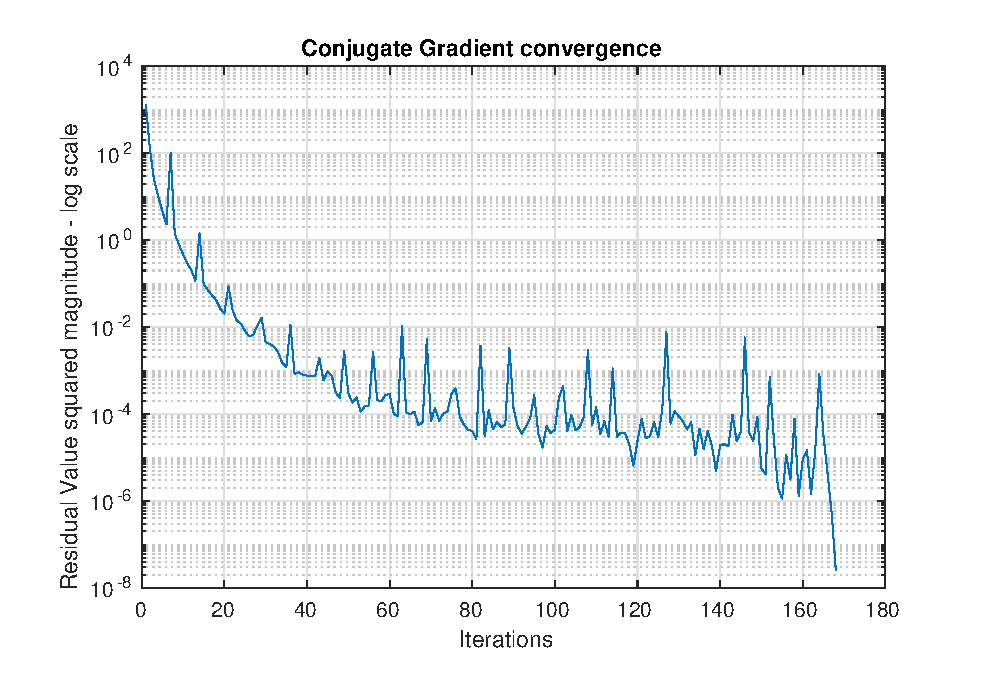
\includegraphics[width=\textwidth, trim={3cm 3cm 3cm 1cm}, clip]{./figures/ex3-2.eps}
% \end{figure}

% The matlab script is contained in \textit{code/ex3\_2.m} file. \newline
% The behavior of the isolines $\propto \mu$ parameter that affects the steepness of the function in the y-dimension.
% For $\mu = 1$, the isolines are circular, indicating that the function increases evenly in all directions from the origin.
% A symmetric paraboloid from the origin is the result of our isotropic quadratic function where its coefficients
% are equal, resulting in a radially symmetric growth.
% For $\mu = 10$, the isolines are ellipses because the function grows faster on the y-dimension resulting in a paraboloid
% steeper along the y-axis and flatter on the x-axis. 
% This behavior is due to the scalar coefficient $\mu$.
% Generally, the isolines indicates how the function behave in the space: 
% closer contour lines mean that the function changes rapidly. 

% \subsection{}
% Considering that $A$ is a symmetric positive-definite matrix, find the exact optimal step-length $\alpha$.
% Show your computations.\newline

% Recalling the formula to compute the step length in ideal case for quadratic forms:
% \myex{
%     \alpha_k = \frac{\nabla f_k^T \nabla f_k}{\nabla f_k^T A \nabla f_k}
% }
% Note that $A$ is SPD $\therefore \, A = A^T$. 
% $A = \myexthreeA$. $\nabla f_k = Ax - b = \myexthreeA \myvec{x \\ y}$ with $b = \vec{0}$. \newline
% By plugging the previously obtained values into the definition:
% \myex{
%     \alpha_k 
%     & = \frac{\nabla f_k^T \nabla f_k}{\nabla f_k^T A \nabla f_k} \\
%     & = \frac{\myvec{x & y} \myexthreeA \myexthreeA \myvec{x \\ y}} 
%             {\myvec{x & y} \myexthreeA \myexthreeA \myexthreeA \myvec{x \\ y}} \\
%     & = \frac{4x^2 + 4 \mu^2 y^2}{8x^2 + 8 \mu^3 y^2} \\
%     & = \frac{1}{2} \cdot \frac{x^2 + \mu^2 y^2}{x^2 + \mu^3 y^2} \\
%     & = \alpha_{opt} \text{ for quadratic forms}
% }
% For $\mu = 1$:
% \myex{
%     \alpha_k 
%     = \frac{1}{2} \cdot \frac{x^2 + y^2}{x^2 + y^2}
%     = \frac{1}{2}
% }
% For $\mu = 10$:
% \myex{
%     \alpha_k 
%     & = \frac{1}{2} \cdot \frac{x^2 + 100 y^2}{x^2 + 1000 y^2} \\
% }

% \subsection{}
% Write a Matlab code for the gradient method with maximum number of iterations $N = 100$ and a tolerance $tol = 10-8$. 
% Minimize $f$ for $\mu = (1, 10)$ and starting points: $(x_0 , y_0) = (10, 0), (0, 10), (10, 10)$. \newline

% The matlab code is contained and extensively documented in the script \textit{code/ex3\_4.m}.
% All the generated plots for the next exercise $3.5$ are done through such script. 

% \subsection{}
% For each case plot the iterations on the energy landscape in 2D (the plot of the objective function),
% the log10 of the norm of the gradient and the value of the energy function (objective function) as functions of the iterations. 
% Comment the results.

% \begin{figure}[H]
%     \centering
%     \caption{Case $\mu = 1, x_0 = (10, 0)$}
%     \label{fig:ex3-5-mu1-x1000}
%     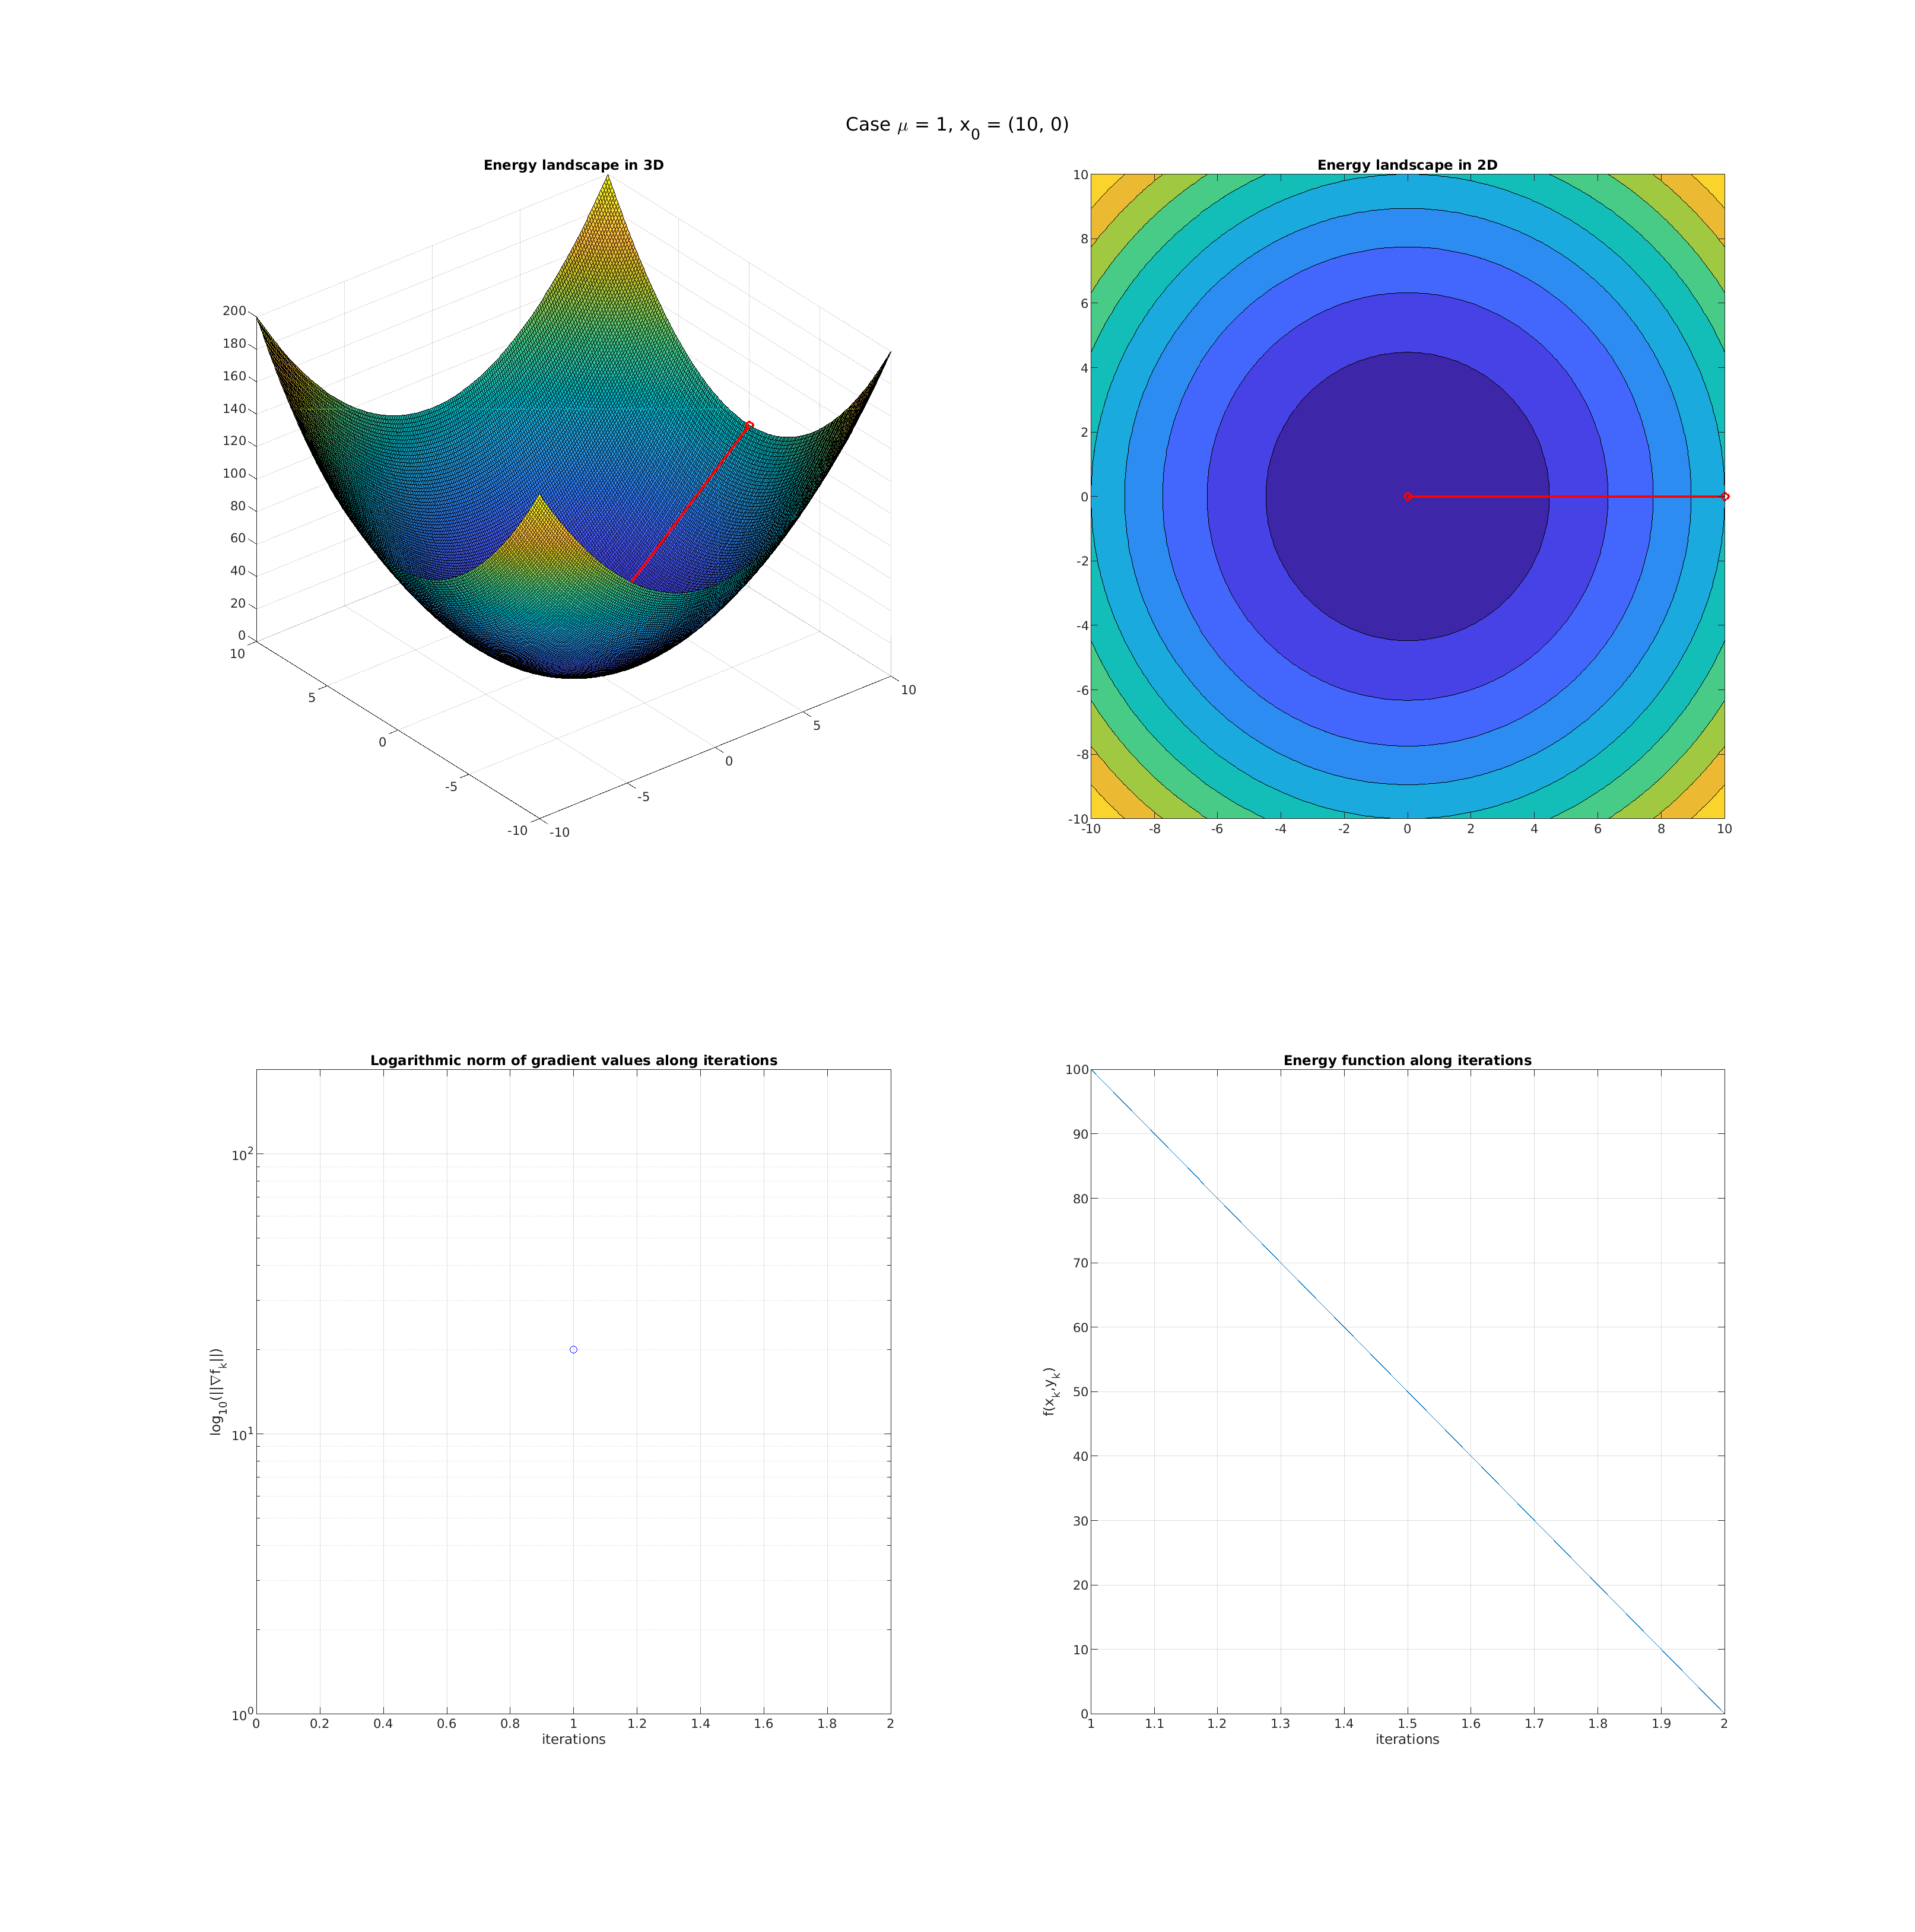
\includegraphics[width=\textwidth, trim={5cm 3cm 5cm 1cm}, clip]{./figures/ex3-5-mu1-x1000.eps}
% \end{figure}

% \begin{figure}[H]
%     \centering
%     \caption{Case $\mu = 1, x_0 = (0, 10)$}
%     \label{fig:ex3-5-mu1-x0010}
%     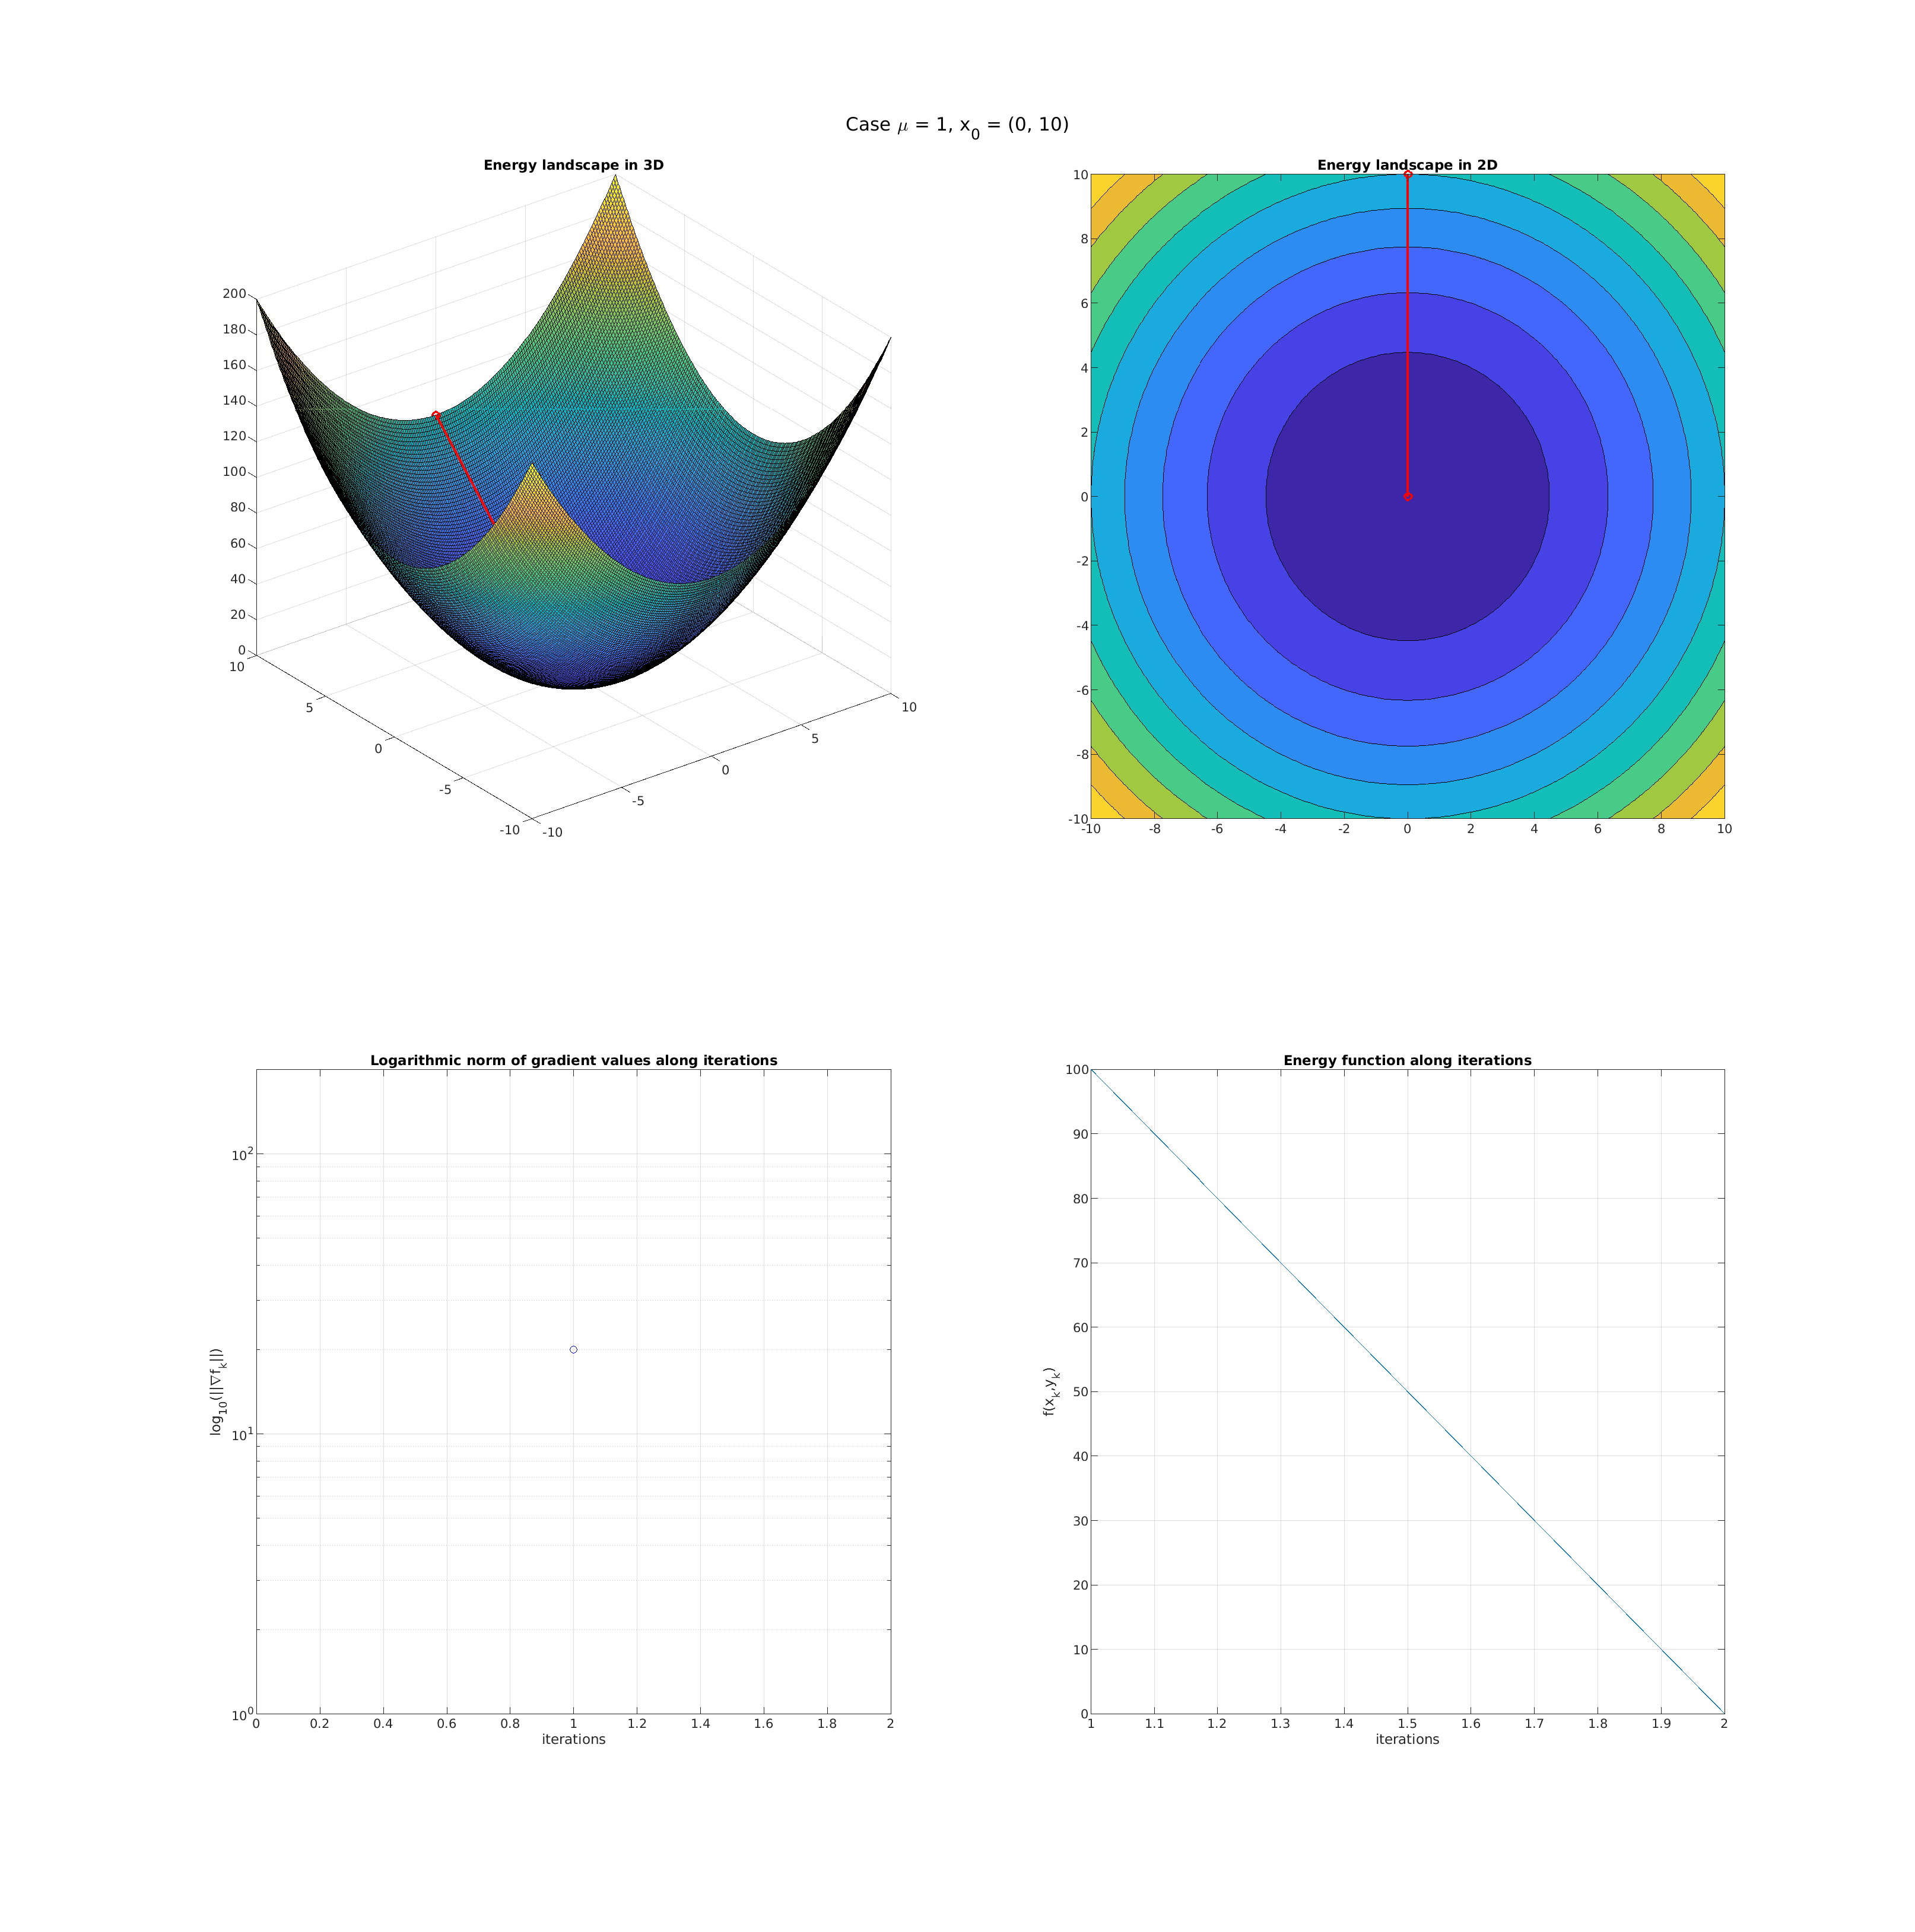
\includegraphics[width=\textwidth, trim={5cm 3cm 5cm 1cm}, clip]{./figures/ex3-5-mu1-x0010.eps}
% \end{figure}

% \begin{figure}[H]
%     \centering
%     \caption{Case $\mu = 1, x_0 = (10, 10)$}
%     \label{fig:ex3-5-mu1-x1010}
%     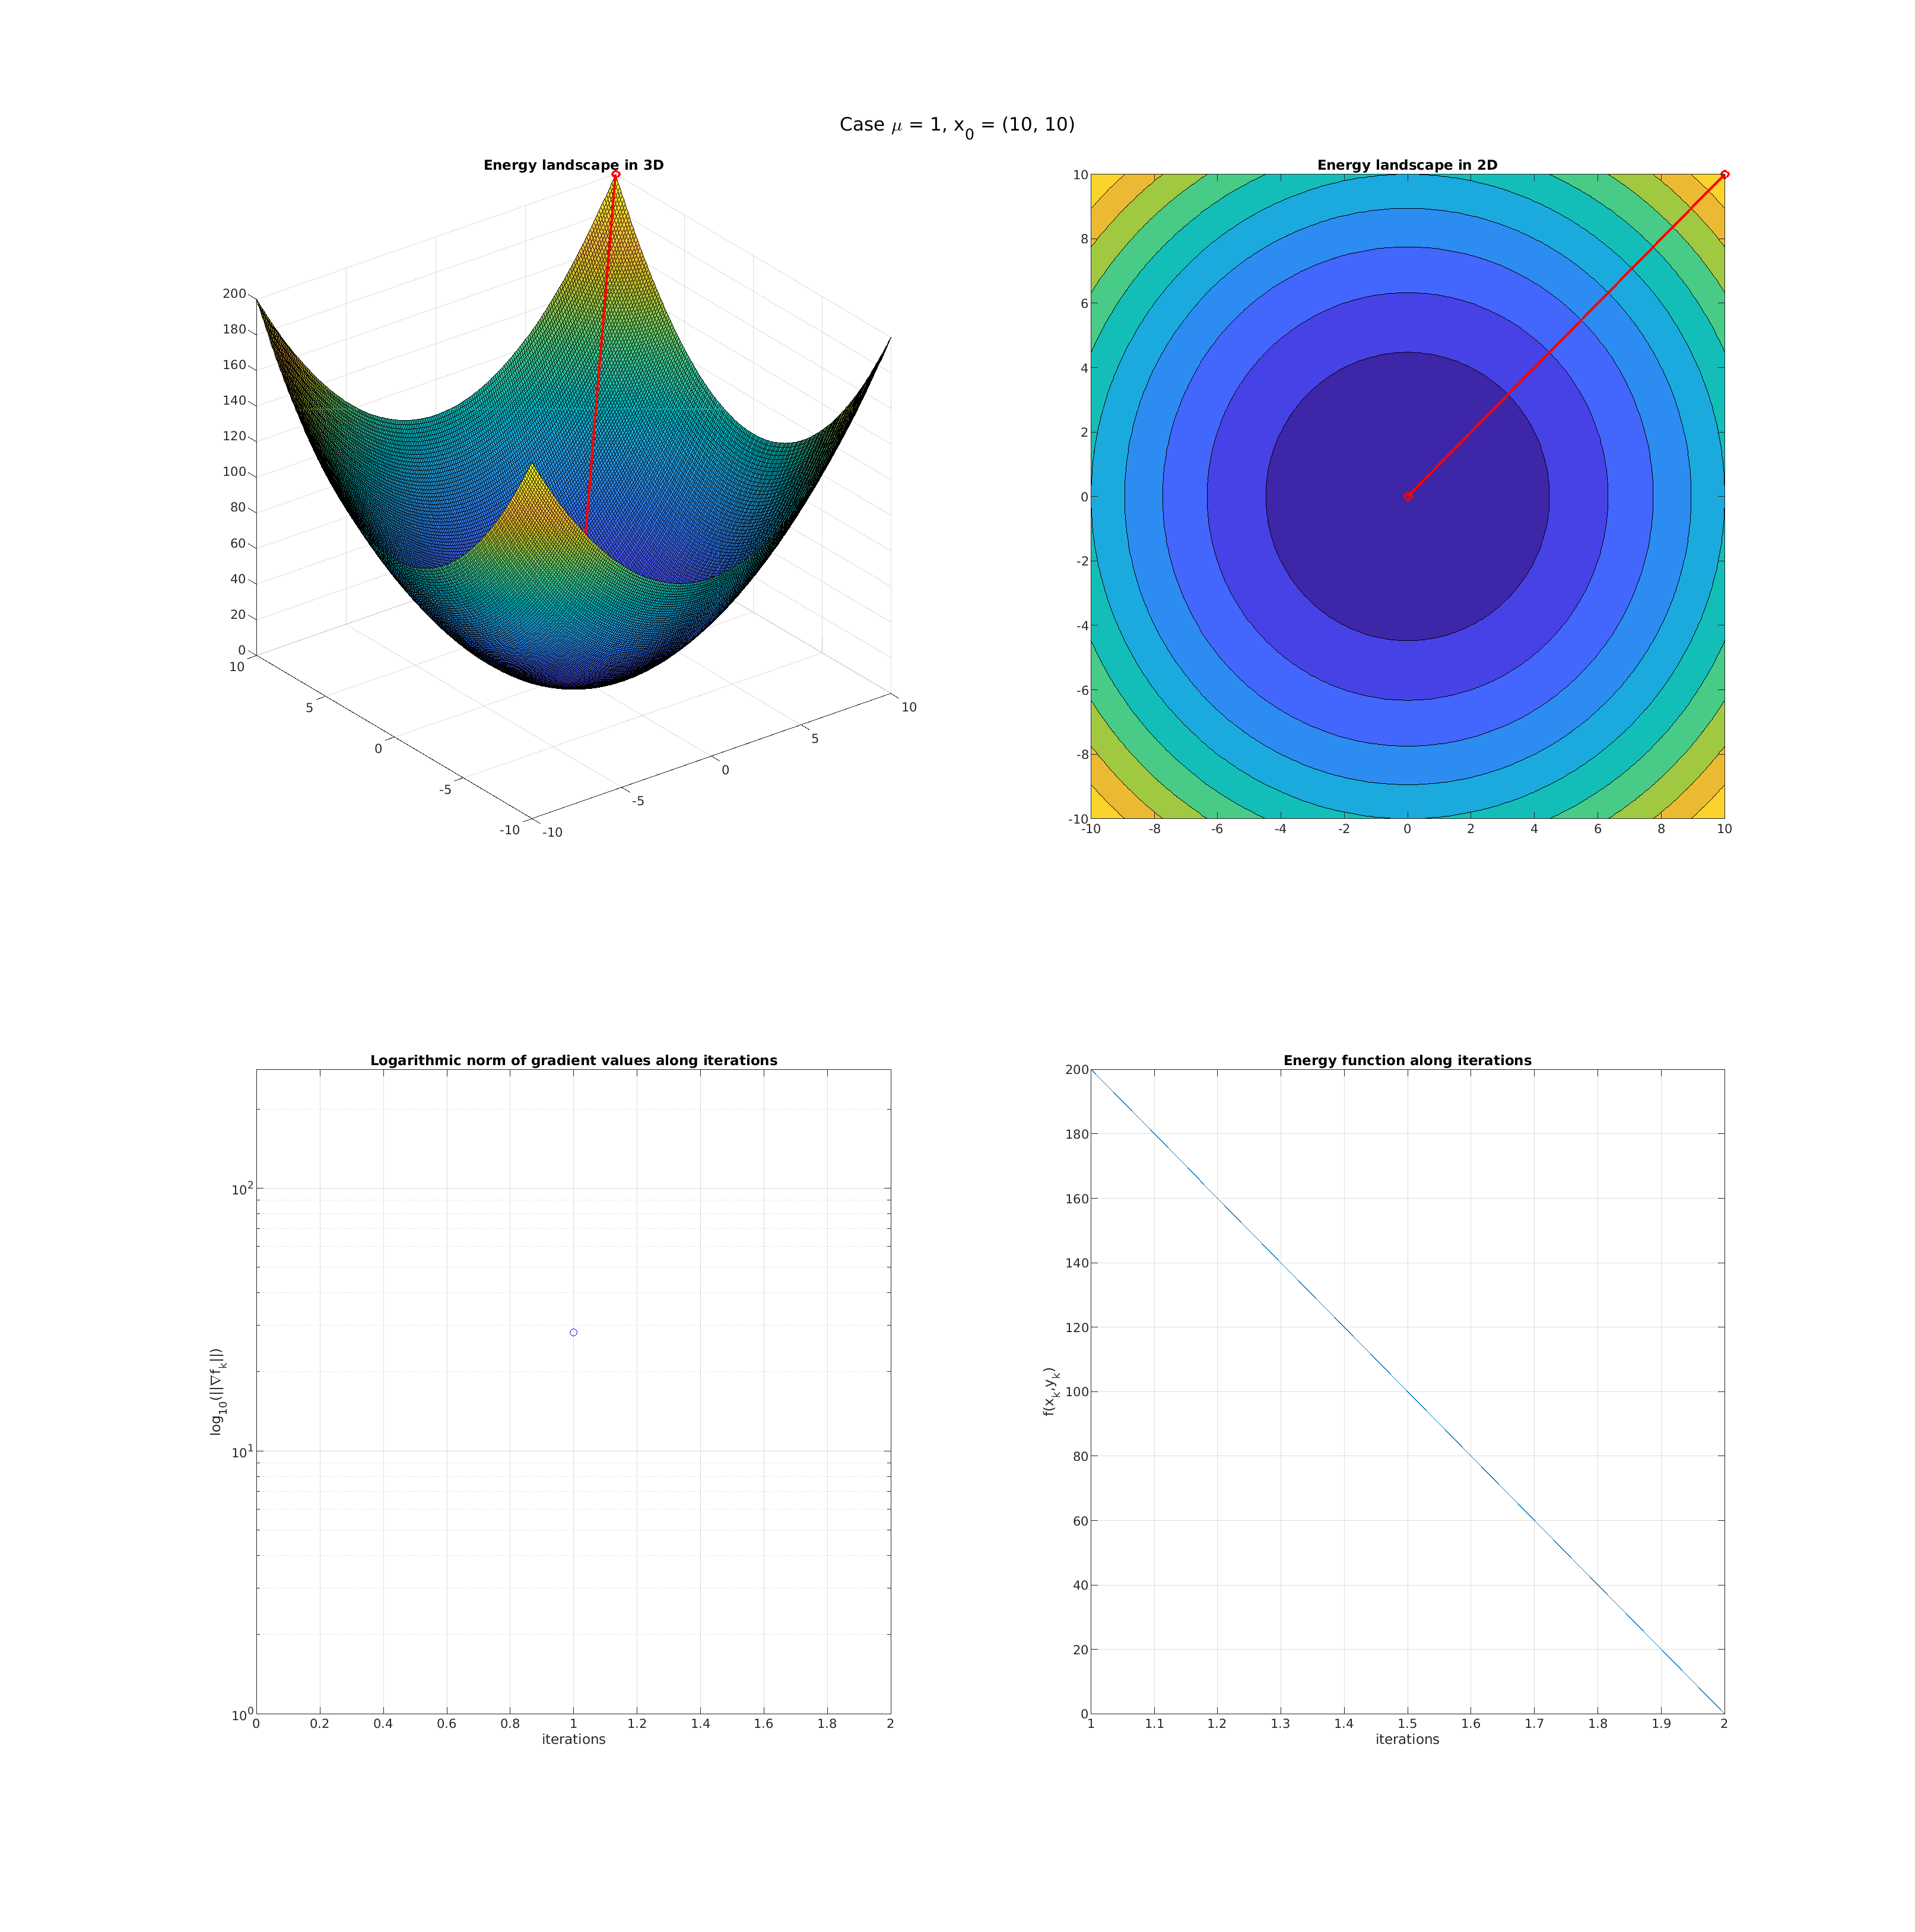
\includegraphics[width=\textwidth, trim={5cm 3cm 5cm 1cm}, clip]{./figures/ex3-5-mu1-x1010.eps}
% \end{figure}

% \begin{figure}[H]
%     \centering
%     \caption{Case $\mu = 10, x_0 = (10, 0)$}
%     \label{fig:ex3-5-mu10-x1000}
%     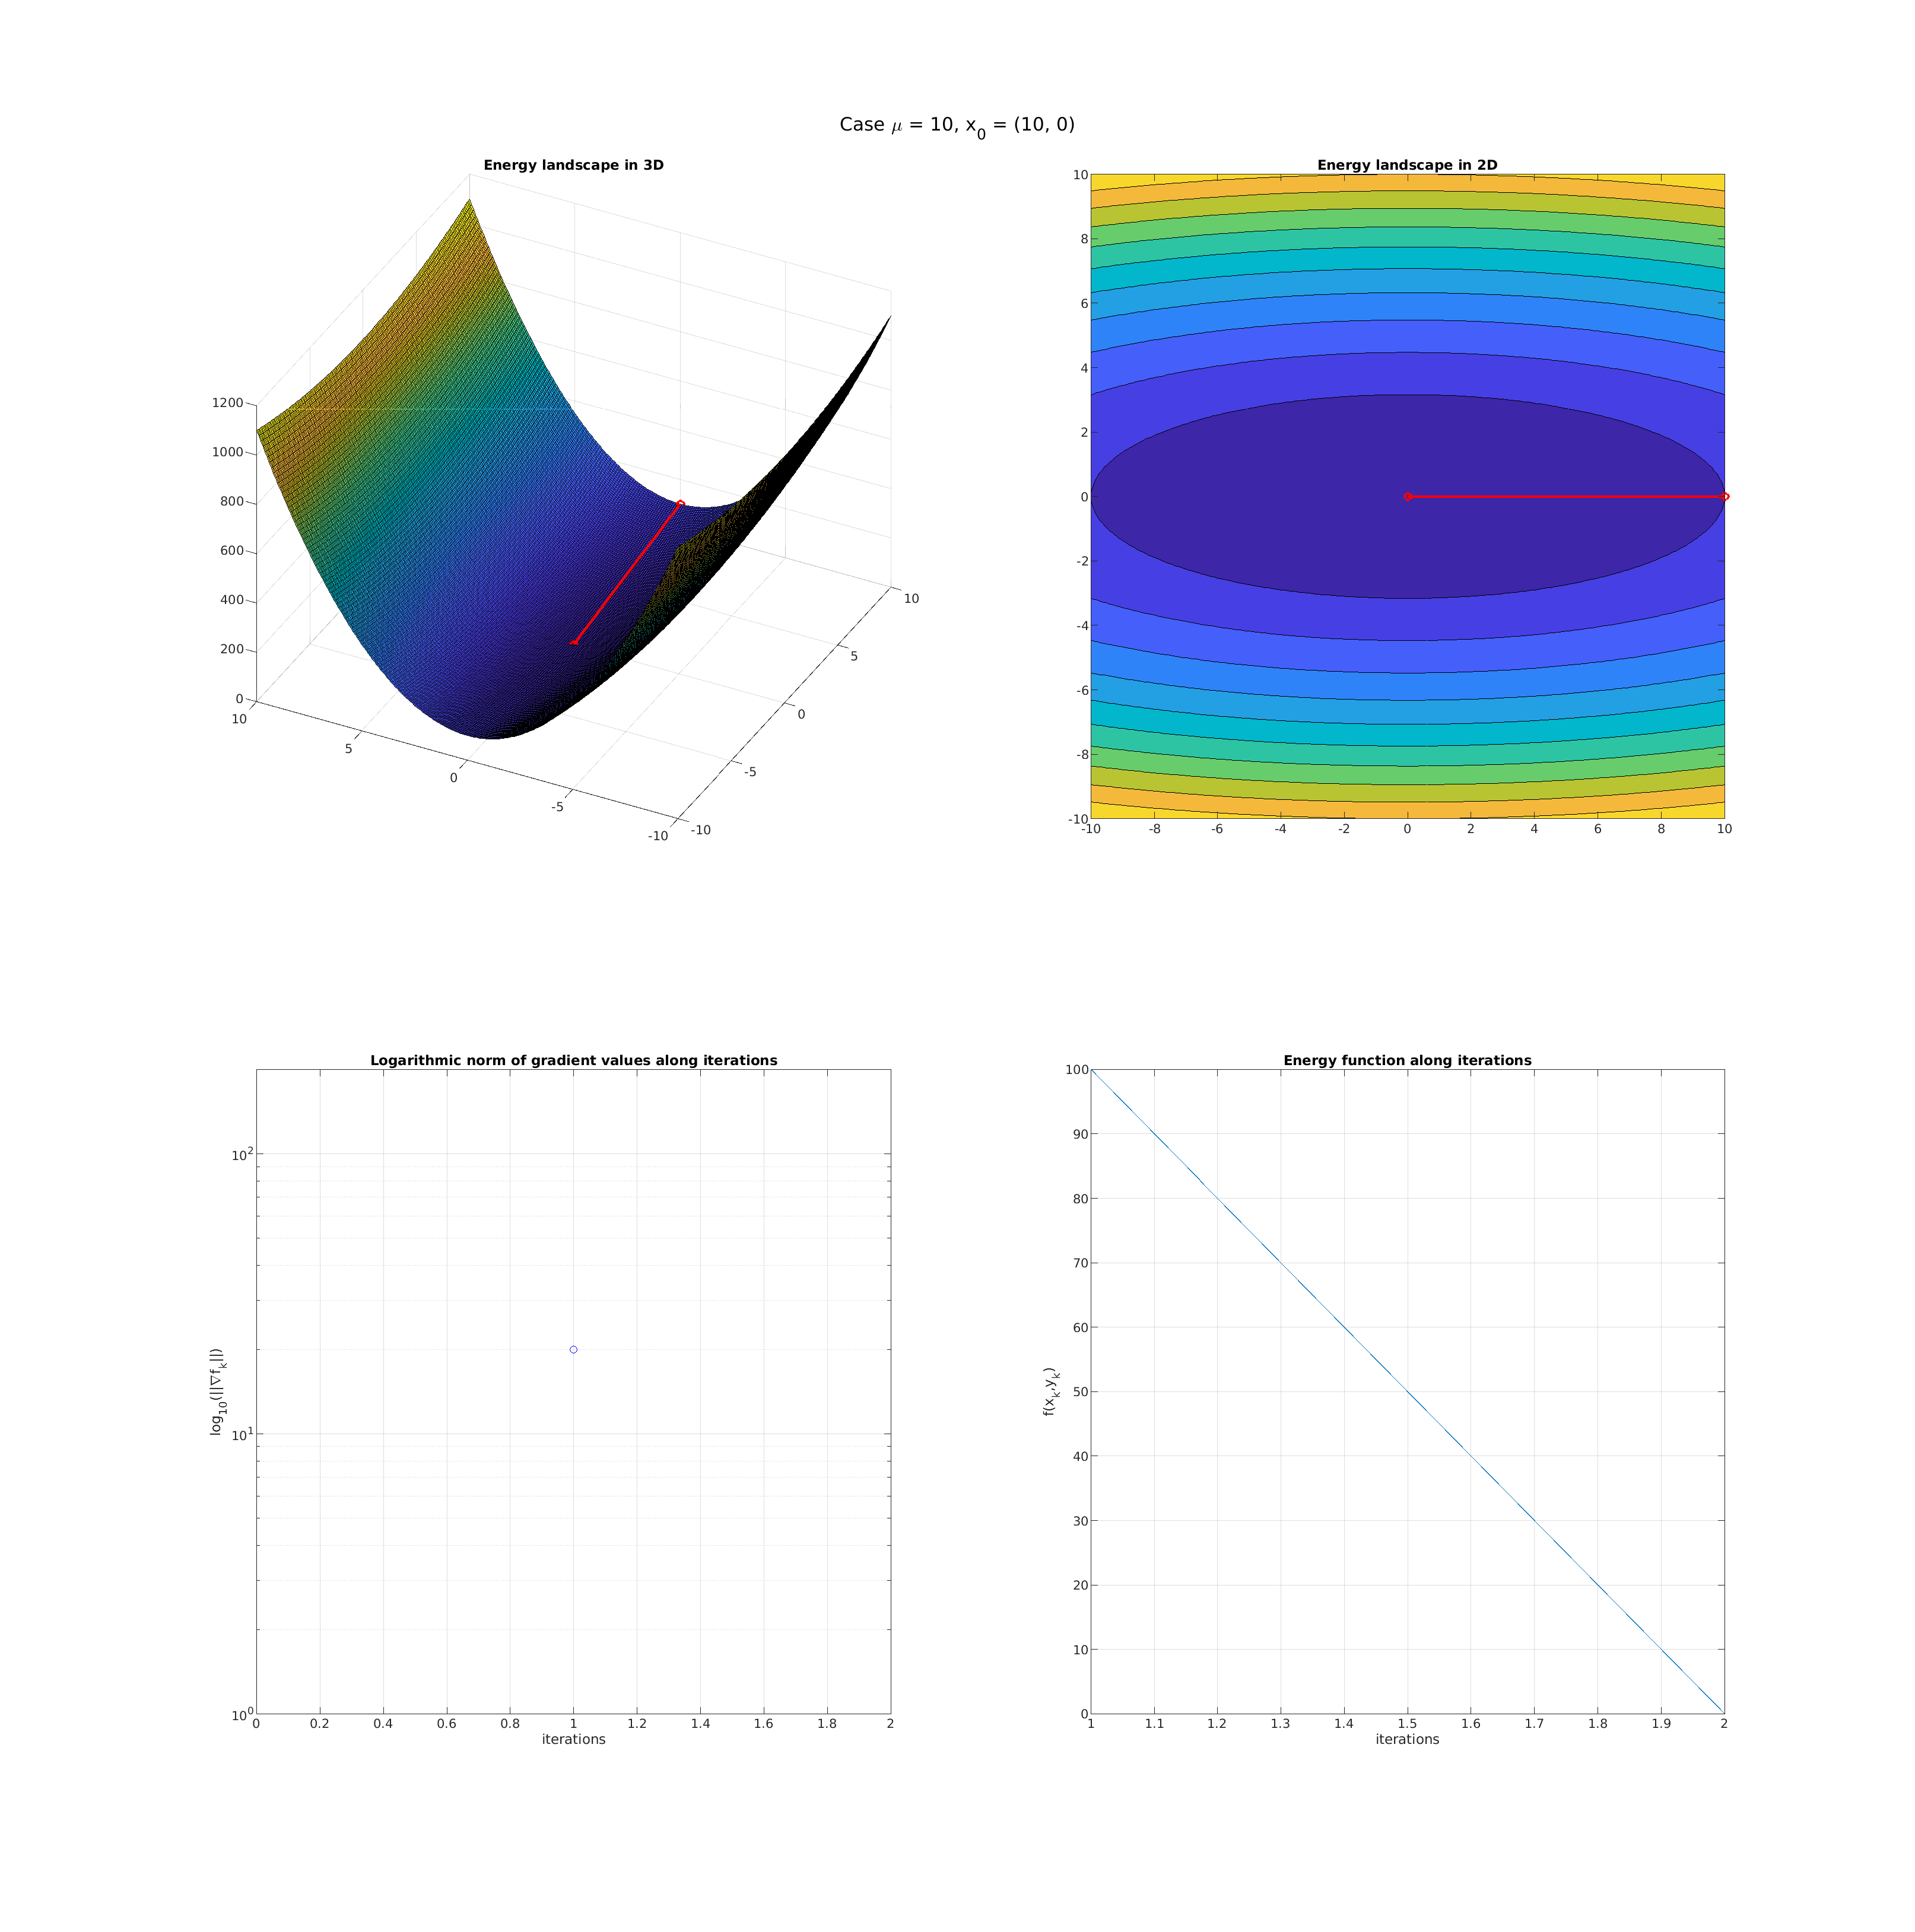
\includegraphics[width=\textwidth, trim={5cm 3cm 5cm 1cm}, clip]{./figures/ex3-5-mu10-x1000.eps}
% \end{figure}

% \begin{figure}[H]
%     \centering
%     \caption{Case $\mu = 10, x_0 = (0, 10)$}
%     \label{fig:ex3-5-mu10-x0010}
%     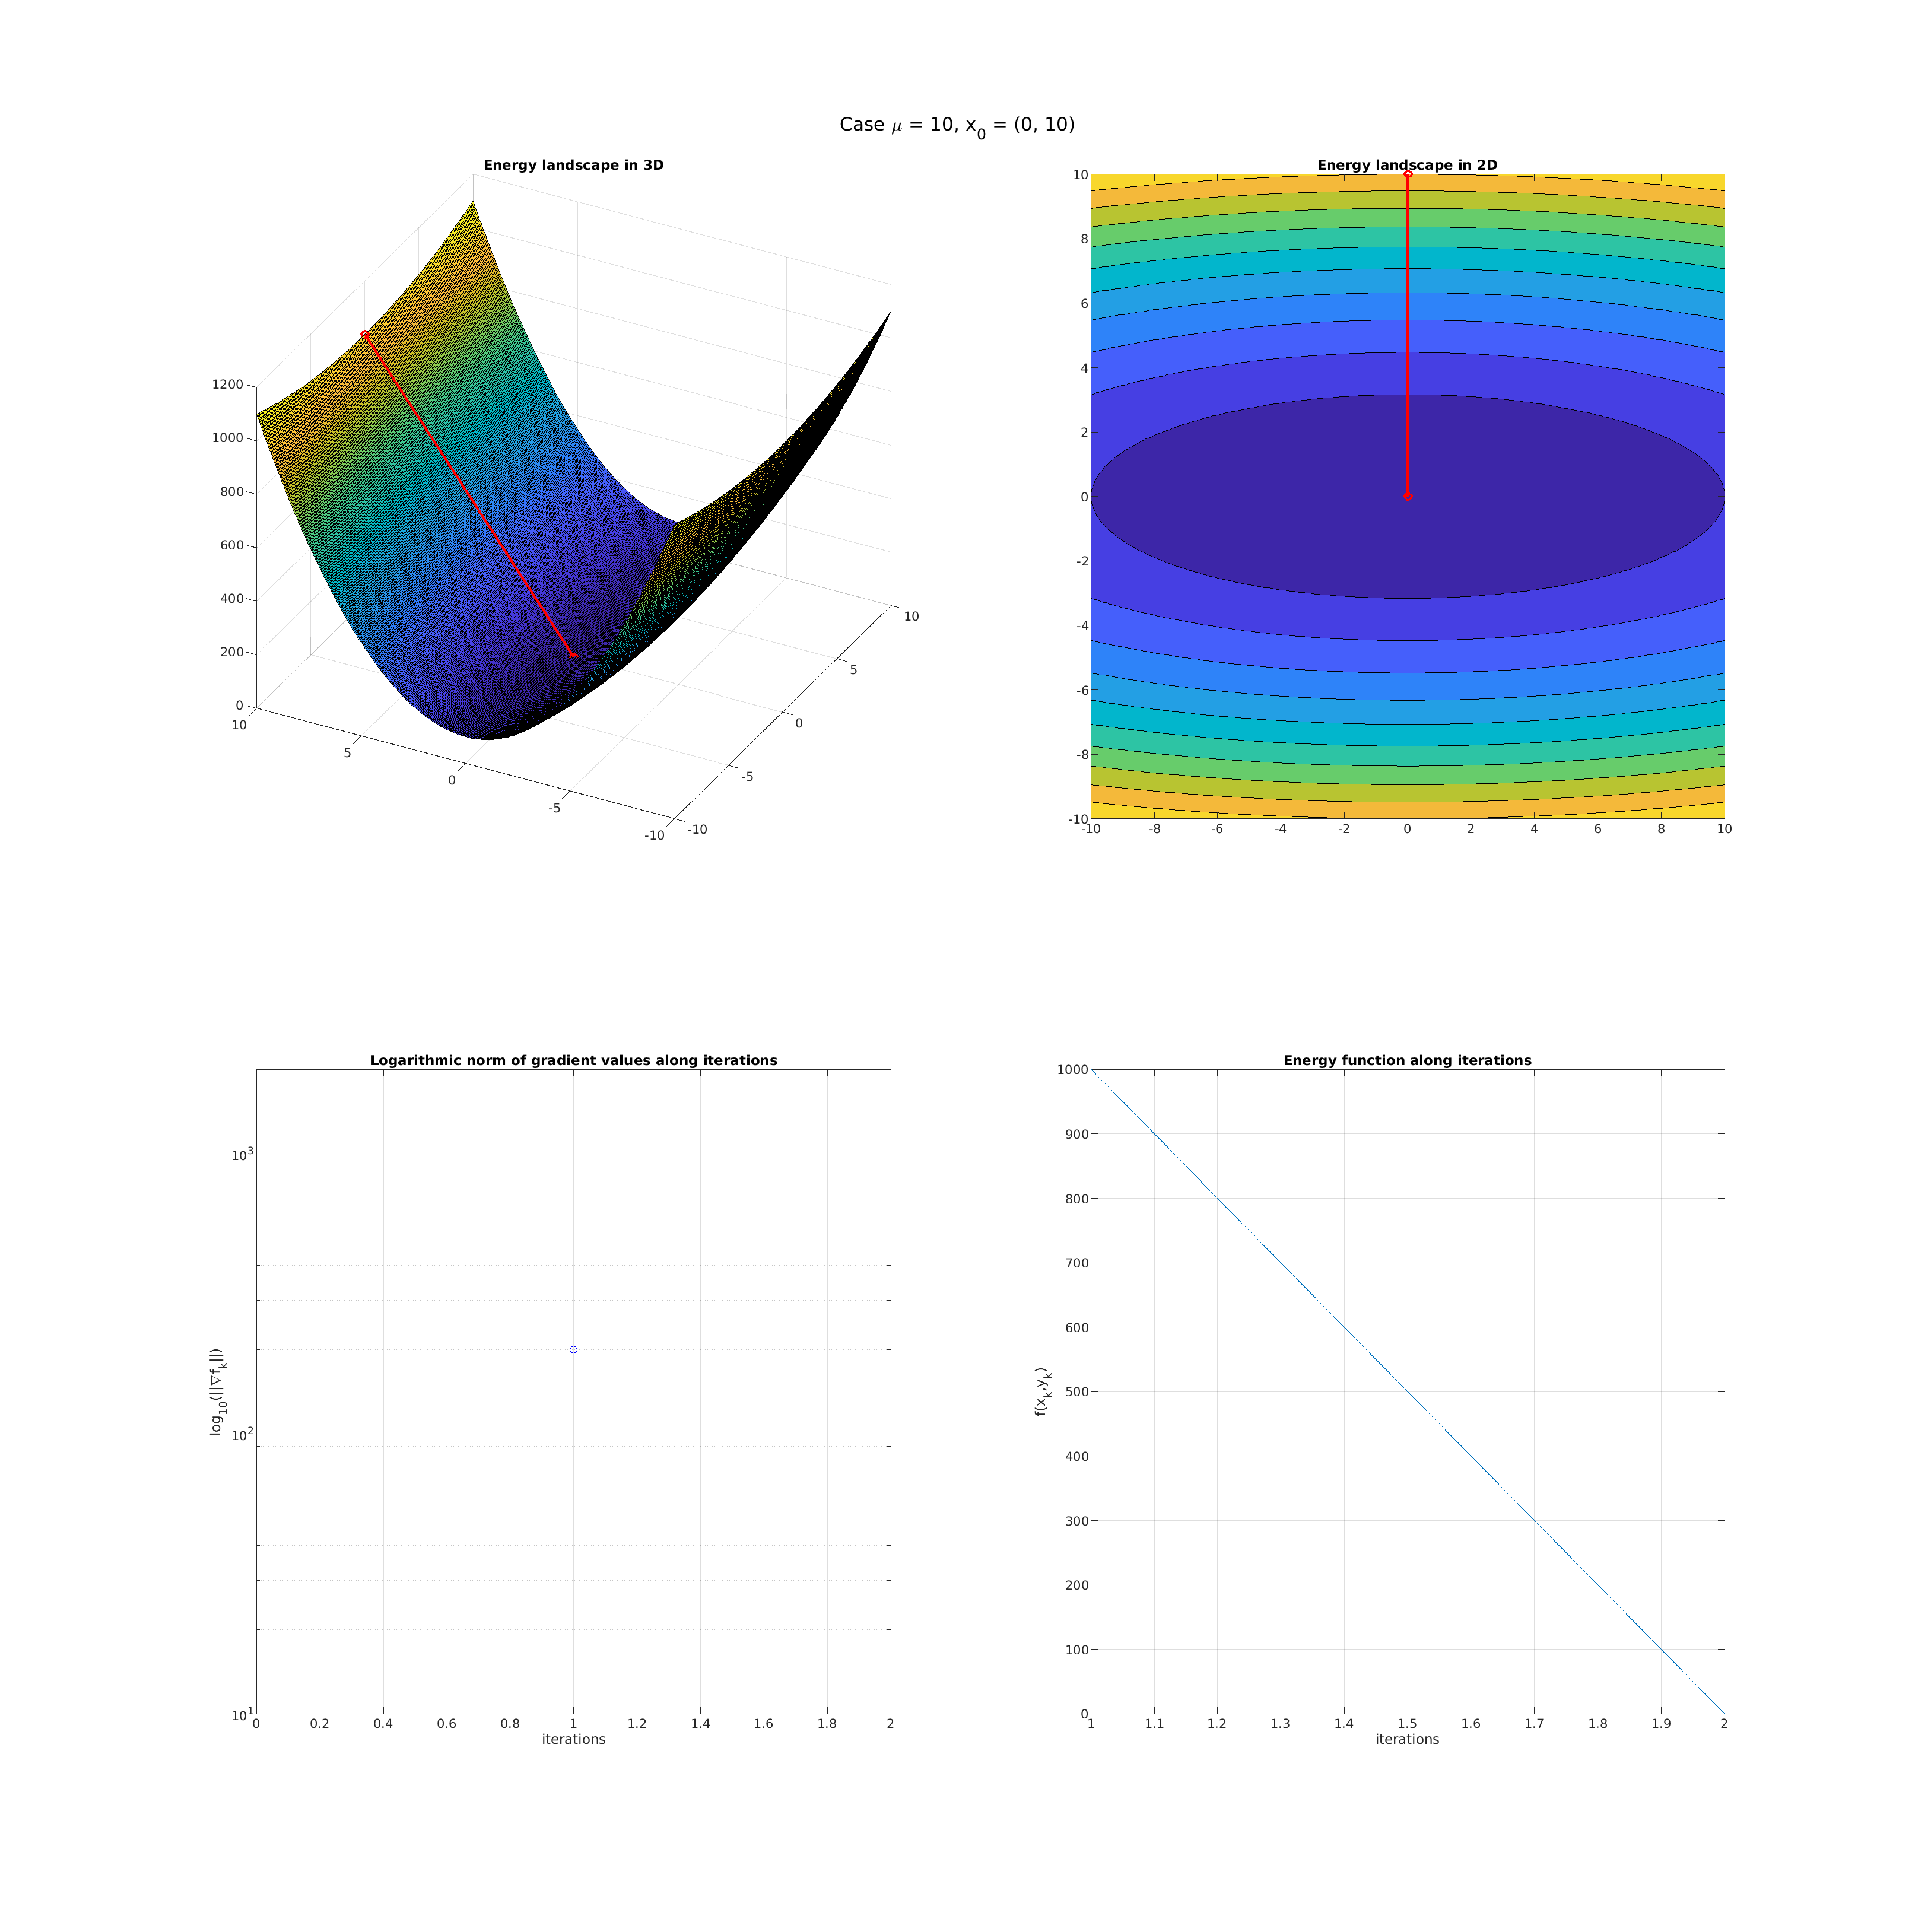
\includegraphics[width=\textwidth, trim={5cm 3cm 5cm 1cm}, clip]{./figures/ex3-5-mu10-x0010.eps}
% \end{figure}

% \begin{figure}[H]
%     \centering
%     \caption{Case $\mu = 10, x_0 = (10, 0)$}
%     \label{fig:ex3-5-mu10-x1010}
%     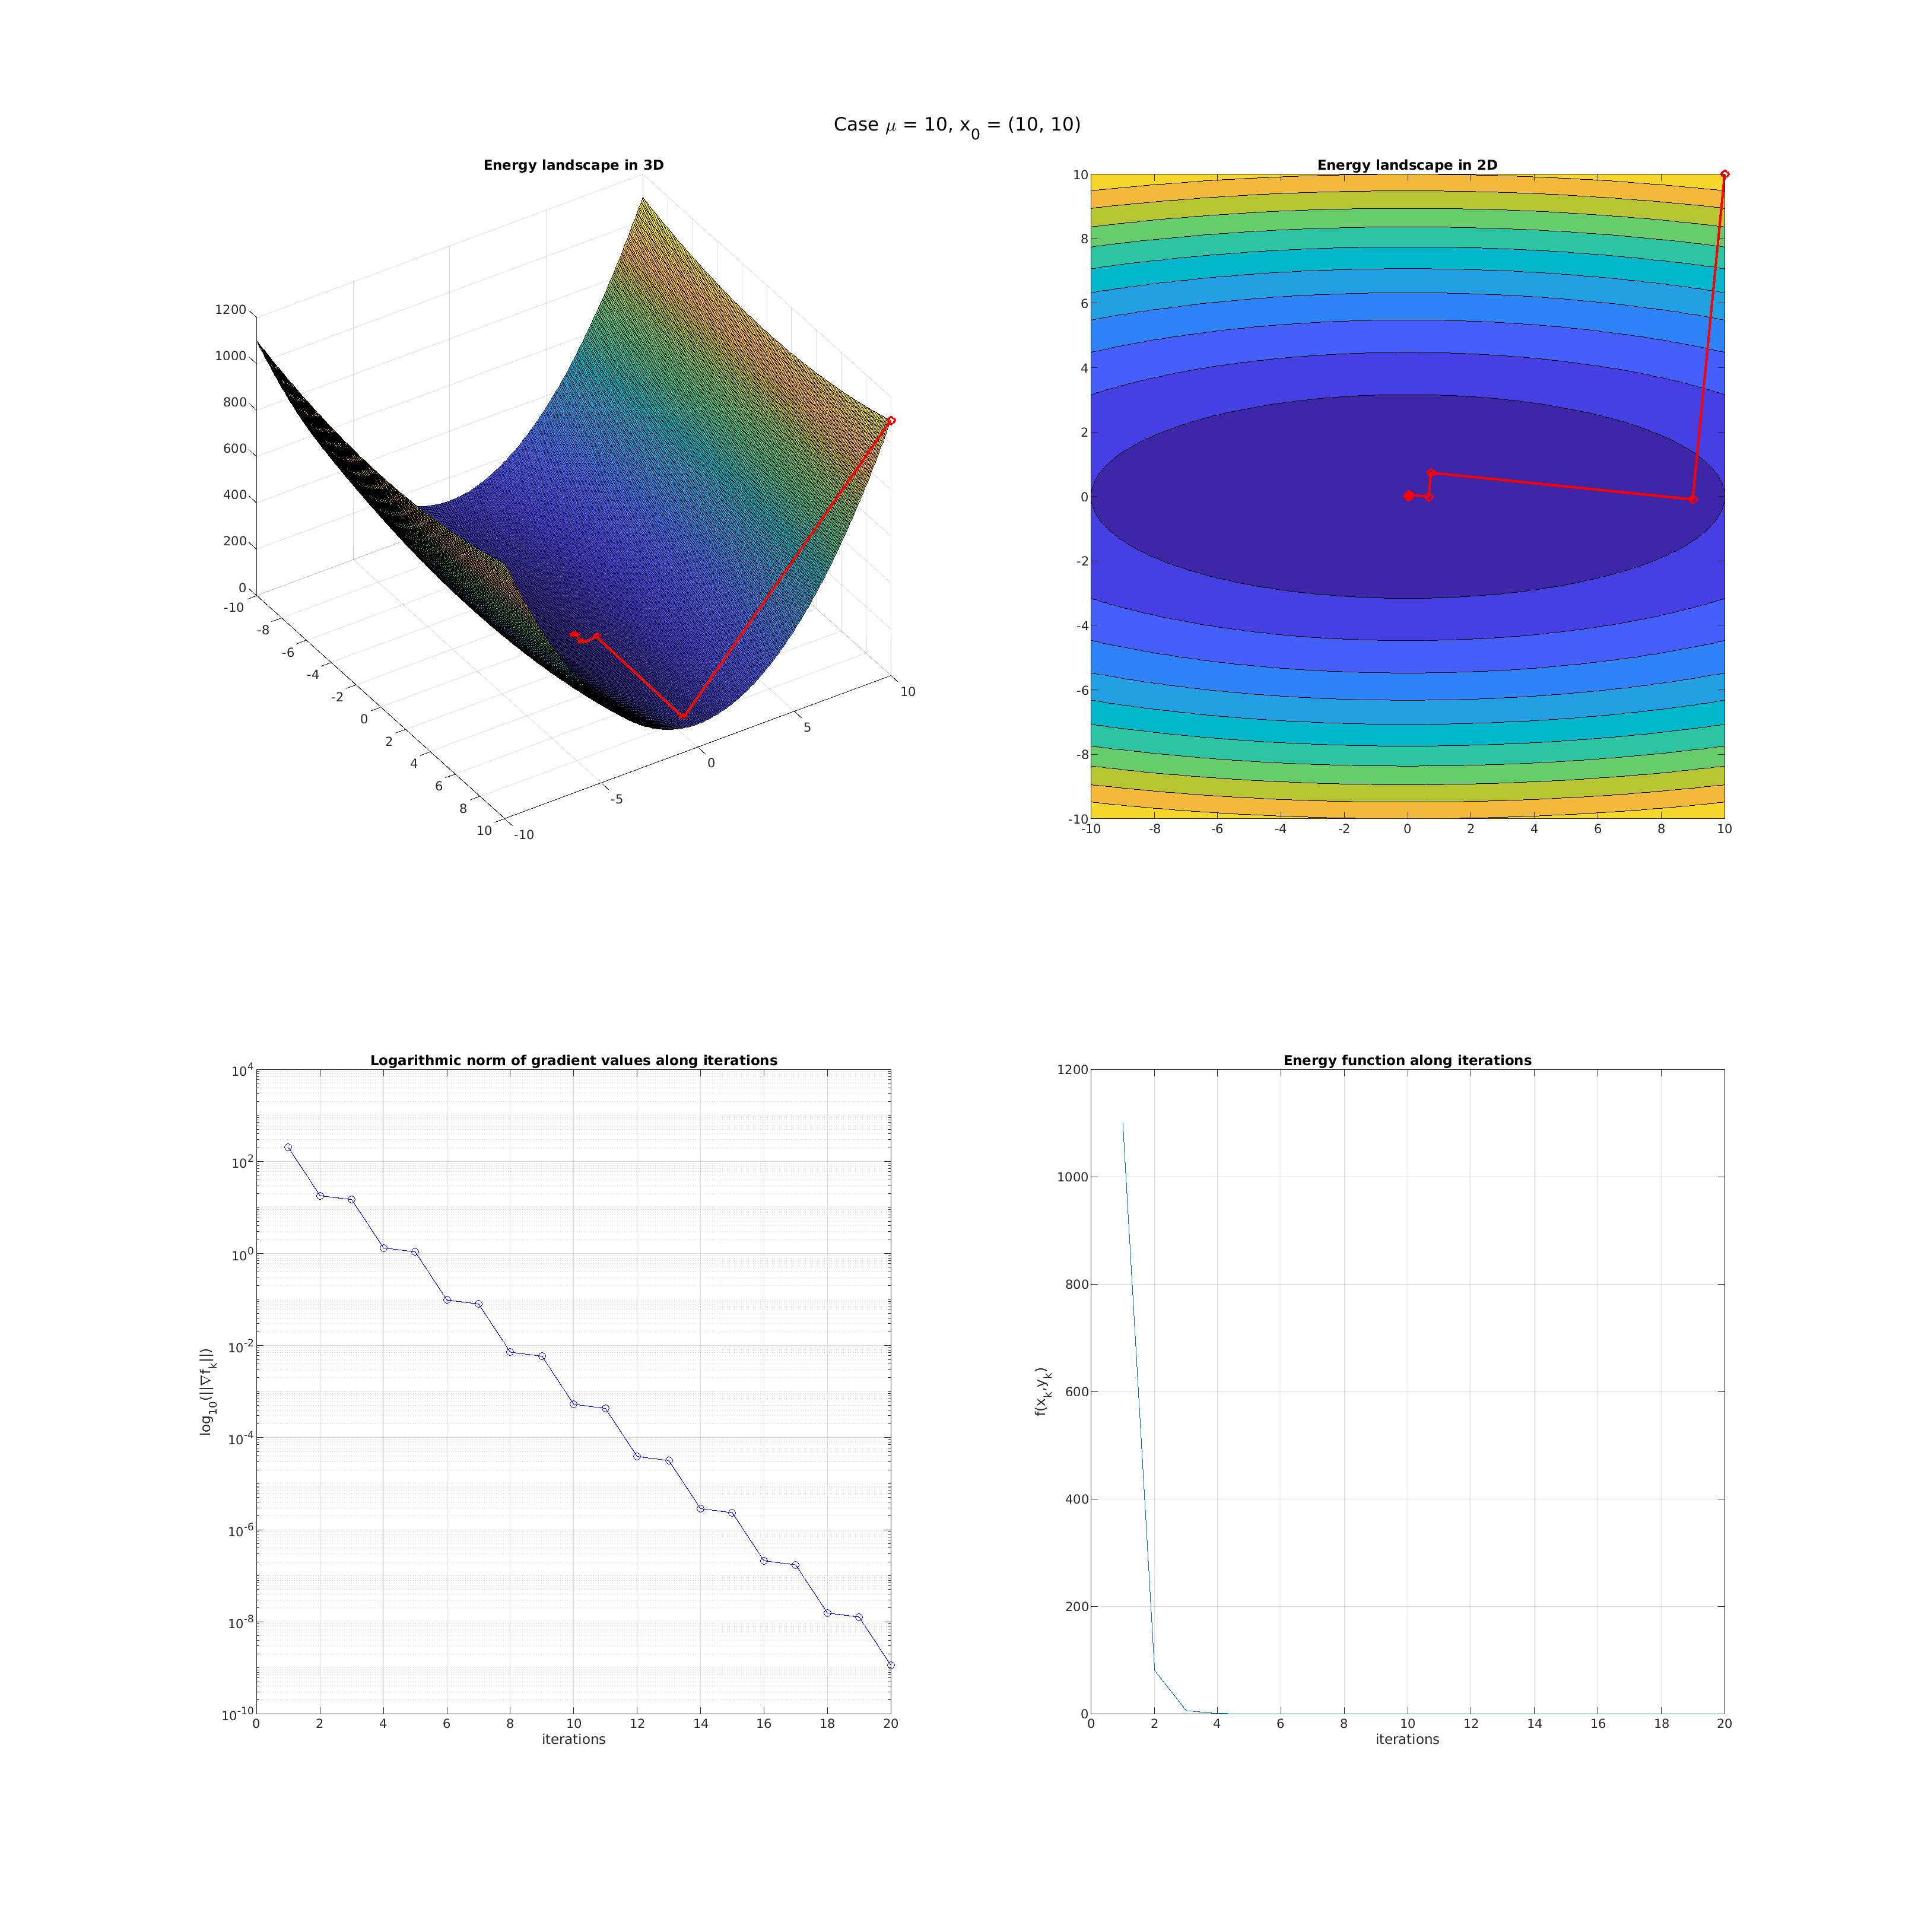
\includegraphics[width=\textwidth, trim={5cm 3cm 5cm 1cm}, clip]{./figures/ex3-5-mu10-x1010.eps}
% \end{figure}

% \textbf{$\mu$ values} \newline
% The parameter $\mu$ can be either the value $1$ or $10$.
% As previously stated in exercise $3.2$, the plots are clustered in 2 groups of 3 samples with respect to 
% $\mu$ value, and whenever it is 1, it's value allows for a radially symmetric expansion of the function 
% as a symmetric paraboloid from the origin which is the local minimizer $x^*$.
% \newline

% \textbf{Convergence \& Isocontours} \newline
% Related to $\mu$ values, isocontours and the energy landscape clearly suggest the change in steepness.
% The convergence of the gradient method is reflected through the isolines and the initial point 
% in every test case since they are important for the method performance.
% Moreover, from Th 3.3 notice that the eigenvalues $\lambda \in \Lambda = spectrum(A)$ for $\mu \neq 1$ are 
% not equal $\lambda_i \neq \lambda_j \text{ for } i \neq j$, meaning that it cannot exploit one-iteration convergence.
% \newline

% \textbf{Number of Iterations} \newline
% For the last plot $\mu = 10, \, x_0 = (10, 0)$, 
% the eigenvalues $\lambda \in \Lambda$ are not all equal and the convergence happens after zigzagging 
% when searching for the local minima.
% This emphasize that the starting point $x_0$ heavily impacts the convergence rate of 
% the steepest descent method,
% despite the function is writable in Quadratic Form and hence strongly convex.

\end{document}
